\newpage
\section{ĐƯỜNG THẲNG VUÔNG GÓC MẶT PHẲNG}
\subsection{LÝ THUYẾT CẦN NHỚ}
\subsubsection{Đường thẳng vuông góc với mặt phẳng}
\begin{dn}
	\immini{
		Đường thẳng $d$ được gọi là vuông góc với mặt phẳng $(\alpha)$ nếu nó vuông góc với mọi đường thẳng $a$ nằm trong mặt phẳng $(\alpha)$.\\
		\textbf{\textit{Ký hiệu:}} $d \perp (\alpha) \Leftrightarrow d \perp a$, $\forall a \subset (\alpha)$.\\
		\textbf{\textit{Nhận xét:}} $\heva{&d \perp (\alpha)\\&a \subset (\alpha)} \Rightarrow d \perp a$.}
	{
		\begin{tikzpicture}[scale=0.7, font=\footnotesize, line join=round, line cap=round, >=stealth]
			\coordinate (A) at (2,2.5);
			\coordinate (B) at (8,2.5);
			\coordinate (D) at (0,0);
			\coordinate (C) at ($(B)+(D)-(A)$);
			\coordinate[label=left:$d$](K) at (3,4);
			\coordinate (P) at (3,1.5);
			\draw [fill=black](P) circle (0.05);
			\coordinate (Q) at (3,0);
			\coordinate (Z) at (3,-1);
			\coordinate (a1) at (3.5,1);
			\coordinate [label=above left:$a$](a2) at (7,1.8);
			\draw(A)--(B)--(C)--(D)--cycle  (K)--(P) (Z)--(Q) (a1)--(a2);
			\draw[dashed]  (P)--(Q);
			\draw pic["$\alpha$",draw,angle eccentricity=0.5, angle radius=0.6cm]{angle=C--D--A};
		\end{tikzpicture}
	}
\end{dn}

\begin{dl}
	\immini{
		Nếu đường thẳng $d$ vuông góc với hai đường thẳng cắt nhau $a$ và $b$ cùng nằm trong mặt phẳng $(\alpha)$ thì $d \perp (\alpha)$.
		$$
		\heva{
			&d \perp a \subset (\alpha) \\
			&d \perp b \subset (\alpha) \\
			&a \cap b = M
		}
		\Rightarrow d \perp (\alpha).
		$$
	}
	{
		\begin{tikzpicture}[scale=0.7, font=\footnotesize, line join=round, line cap=round, >=stealth]
			\coordinate (A) at (2,2.5);
			\coordinate (B) at (8,2.5);
			\coordinate (D) at (0,0);
			\coordinate (C) at ($(B)+(D)-(A)$);
			\coordinate[label=left:$d$](K) at (3,4);
			\coordinate (P) at (3,1.5);
			\coordinate (P1) at (3,2);
			\coordinate (P2) at (3.5,1.5);
			\draw [fill=black](P) circle (0.05);
			\coordinate (Q) at (3,0);
			\coordinate (Z) at (3,-1);
			\coordinate (a1) at (3.5,1);
			\coordinate [label=above left:$a$](a2) at (7,1.8);
			\coordinate (b1) at (3.7,1.3);
			\coordinate [label=above:$b$](b2) at (6,0.8);
			\coordinate [label=above :$M$] (M) at (intersection of a1--a2 and b1--b2);
			\draw [fill=black](M) circle (0.05);
			\draw(A)--(B)--(C)--(D)--cycle  (K)--(P) (Z)--(Q) (a1)--(a2) (b1)--(b2);
			\draw[dashed]  (P)--(Q);
			\draw pic[draw,angle radius=0.2cm]{right angle=P1--P--P2};
			\draw pic["$\alpha$",draw,angle eccentricity=0.55, angle radius=0.6cm]{angle=C--D--A};
		\end{tikzpicture}
	}
\end{dl}

\begin{dl}
	\begin{itemize}
	\item Có duy nhất một mặt phẳng đi qua một điểm và vuông góc với một đường thẳng cho trước.
	\item Có duy nhất một đường thẳng đi qua một điểm và vuông góc với một mặt phẳng cho trước.
	\end{itemize}
\end{dl}
\subsubsection*{Mặt phẳng trung trực của một đoạn thẳng}
\begin{dn}
	\immini{
		Mặt phẳng đi qua trung điểm $I$ của đoạn thẳng $AB$ và vuông góc với đường thẳng $AB$ là mặt phẳng trung trực của đoạn thẳng $AB$.\\
		\textbf{Nhận xét:} $(P)$ là mặt phẳng trung trực của đoạn thẳng $AB \Leftrightarrow \forall M \in (P)$, $MA = MB$.}
	{
		\begin{tikzpicture}[scale=0.7, font=\footnotesize, line join=round, line cap=round, >=stealth]
			\coordinate (A1) at (0,5);
			\coordinate (B1) at (3,6.7);
			\coordinate (D1) at (0,0);
			\coordinate (C1) at ($(B1)+(D1)-(A1)$);
			\coordinate (I) at (1.5,3);
			\coordinate (A) at (-2.5,3);
			\coordinate (B) at (5,3);
			\coordinate (I2) at (intersection of A--I and A1--D1);
			\coordinate (M) at (2.3,5.5);
			\coordinate (M2) at (intersection of A--M and A1--D1);
			\draw(A1)--(B1)--(C1)--(D1)--cycle (A)--(I2) (I)--(B) (A)--(M2) (I)--(M)--(B);
			\path (A)--(I) node[midway,sloped]{$/$}	;
			\path (B)--(I) node[midway,sloped]{$/$};
			\draw [dashed] (I2)--(I) (M2)--(M);
			\draw pic["$P$",draw,angle eccentricity=0.5, angle radius=0.7cm]{angle=C1--D1--A1};
			\foreach \x/\goc in {I/-90,A/150,B/0,M/90}
			\draw[fill=white] (\x) node[shift={(\goc:7pt)},font=\scriptsize]{$\x$} circle (1pt);
		\end{tikzpicture}
	}
\end{dn}
\subsubsection*{Trục của đa giác}
\begin{dn}
	Trục của đa giác là đường thẳng qua tâm của đường tròn ngoại tiếp đa giác và vuông góc với mặt phẳng chứa đa giác đó. Nếu một điểm nằm trên trục của đa giác thì nó cách đều các đỉnh của đa giác.
	\begin{center}
		\begin{tikzpicture}[scale=0.8,font=\footnotesize, line join=round, line cap=round, >=stealth]
			\path
			(0,0) coordinate (A)
			(5,0) coordinate (C)
			(1,-1.5) coordinate (B)
			($(C)!.5!(B)$) coordinate (N)
			($(A)!2/3!(N)$) coordinate (H)
			($(H)+(0,3)$) coordinate (M)
			($(M)!1.5!(H) $) coordinate (E)
			;
			\coordinate (E1) at (intersection of M--E and B--C);
			\draw (A)--(M) (B)--(M) (M)--(C) (A)--(B)--(C) (E1)--(E);
			\draw[dashed] (A)--(C) (M)--(H) (C)--(H)--(B) (A)--(H)--(E1);
			\path (B)--(M) node[midway,sloped]{$/$};
			\path (C)--(M) node[midway,sloped]{$/$};
			\path (A)--(M) node[midway,sloped]{$/$};
			\fill (E) node[right]{$\Delta$};
			\foreach \x/\goc in {A/180,B/-90,C/0,M/90,H/-35}
			\draw[fill=white] (\x) node[shift={(\goc:7pt)},font=\scriptsize]{$\x$} circle (1pt);
			\node[below=0.1cm, align=center] at (current bounding box.south) {Tam giác thường};
		\end{tikzpicture}\hspace{0.5cm}
		\begin{tikzpicture}[scale=0.8,font=\footnotesize, line join=round, line cap=round, >=stealth]
			\path
			(0,0) coordinate (A)
			(5,0) coordinate (C)
			(1,-1.5) coordinate (B)
			($(C)!.5!(B)$) coordinate (N)
			($(A)!2/3!(N)$) coordinate (H)
			($(H)+(0,3)$) coordinate (M)
			($(M)!1.5!(H) $) coordinate (E)
			;
			\coordinate (E1) at (intersection of M--E and B--C);
			\coordinate (B1) at (intersection of B--H and A--C);
			\draw (A)--(B)--(C)--(A) (E1)--(E) (M)--(E);
			\draw[dashed]  (C)--(H)--(B) (A)--(H)--(B1);
			\path (B)--(H) node[midway,sloped]{$|$};
			\path (C)--(H) node[midway,sloped]{$|$};
			\path (A)--(H) node[midway,sloped]{$|$};
			\fill (M) node[right]{$\Delta$};
			\draw pic[draw,angle radius=0.25cm]{right angle=H--B1--C};
			\foreach \x/\goc in {A/180,B/-90,C/0,H/-35}
			\draw[fill=white] (\x) node[shift={(\goc:7pt)},font=\scriptsize]{$\x$} circle (1pt);
			\node[below=0.1cm, align=center] at (current bounding box.south) {Tam giác đều};
		\end{tikzpicture}\hspace{0.5cm}
		\begin{tikzpicture}[scale=0.8,font=\footnotesize, line join=round, line cap=round, >=stealth]
			\path
			(0,0) coordinate (A)
			(5,0) coordinate (C)
			(1,-1.5) coordinate (B)
			($(C)!.5!(B)$) coordinate (N)
			($(A)!.5!(C)$) coordinate (H)
			($(H)+(0,3)$) coordinate (M)
			($(M)!1.5!(H) $) coordinate (E)
			;
			\coordinate (E1) at (intersection of M--E and B--C);
			\coordinate (B1) at (intersection of B--H and A--C);
			\draw (A)--(B)--(C)--(A) (H)--(B)  (M)--(H) (E1)--(E);
			\draw[dashed]  (H)--(E1);
			\path (B)--(H) node[midway,sloped]{$|$};
			\path (C)--(H) node[midway,sloped]{$|$};
			\path (A)--(H) node[midway,sloped]{$|$};
			\fill (M) node[right]{$\Delta$};
			\draw pic[draw,angle radius=0.25cm]{right angle=A--H--M};
			\draw pic[draw,angle radius=0.25cm]{right angle=A--B--C};
			\foreach \x/\goc in {A/180,B/-90,C/0,H/45}
			\draw[fill=white] (\x) node[shift={(\goc:7pt)},font=\scriptsize]{$\x$} circle (1pt);
			\node[below=0.1cm, align=center] at (current bounding box.south) {Tam giác vuông};
		\end{tikzpicture}
	\end{center}
	\textbf{\textit{Chứng minh:}}\\
	Cho đa giác có $n$ đỉnh $A_1, A_2, \dots, A_n$.\\
	Gọi $O$ là tâm đường tròn ngoại tiếp đa giác và $d$ là trục của đa giác.\\
	Lấy điểm $I \in d$.\\
	Khi đó $\triangle IOA_1 = \triangle IOA_2 = \dots = \triangle IOA_n$ (các tam giác vuông có hai cạnh bằng nhau) $\Rightarrow IA_1 = IA_2 = \dots = IA_n$.
\end{dn}
\subsubsection{Liên hệ giữa tính song song và tính vuông góc của đường thẳng và mặt phẳng}
\begin{dl}
	\immini{
		\begin{enumerate}[a)]
			\item Cho hai đường thẳng song song. Mặt phẳng nào vuông góc với đường thẳng này thì cũng vuông góc với đường thẳng kia.\\
			\textbf{\textit{Tóm tắt }}$\heva{&a \parallel b \\&a \perp (\alpha)
			}\Rightarrow b \perp (\alpha)$.
			\item Hai đường thẳng phân biệt cùng vuông góc với một mặt phẳng thì song song với nhau.\\
			\textbf{\textit{Tóm tắt }}$\heva{&a \neq b \\&a \perp (\alpha) \\&b \perp (\alpha)}\Rightarrow a \parallel b$.
		\end{enumerate}
	}
	{
		\begin{tikzpicture}[scale=0.65, font=\footnotesize, line join=round, line cap=round, >=stealth]
			\coordinate (A) at (1.5,3);
			\coordinate (B) at (6.5,3);
			\coordinate (D) at (0,0);
			\coordinate[label=left:$a$](E) at (2,4) ;
			\coordinate (F) at (2,1.5);
			\coordinate (M) at (2,0);
			\coordinate (N) at (2,-1);
			\coordinate[label=left:$b$](K) at (4,4);
			\coordinate (P) at (4,1.5);
			\coordinate (Q) at (4,0);
			\coordinate (Z) at (4,-1);
			\coordinate (C) at ($(B)+(D)-(A)$);
			\draw(A)--(B)--(C)--(D)--cycle (E)--(F) (M)--(N) (K)--(P) (Z)--(Q);
			\draw[dashed] (F)--(M) (P)--(Q);
			\draw pic[draw,angle radius=0.2cm]{right angle=E--F--P};
			\draw pic[draw,angle radius=0.2cm]{right angle=K--P--F};
			\draw pic["$\alpha$",draw,angle eccentricity=0.5, angle radius=0.5cm]{angle=C--D--A};
		\end{tikzpicture}
	}
\end{dl}

\begin{dl}
	\immini{
		\begin{enumerate}[a)]
			\item Cho hai mặt phẳng song song. Đường thẳng nào vuông góc với mặt phẳng này thì cũng vuông góc với mặt phẳng kia.\\
			\textbf{Tóm tắt} $\heva{&(\alpha)\parallel (\beta)\\ &a \perp (\alpha)}\Rightarrow a \perp (\beta)$.
			\item Hai mặt phẳng phân biệt cùng vuông góc với một đường thẳng thì song song với nhau.\\
			\textbf{Tóm tắt} $\heva{& (\alpha)\ne (\beta)\\ &(\alpha)\perp a\\ &(\beta) \perp a}\Rightarrow (\alpha)\parallel (\beta)$.
		\end{enumerate}
	}
	{
		\begin{tikzpicture}[scale=0.65, font=\footnotesize, line join=round, line cap=round, >=stealth]
			\coordinate (A) at (1.5,2.5);
			\coordinate (B) at (7.5,2.5);
			\coordinate (D) at (0,0);
			\coordinate (C) at ($(B)+(D)-(A)$);
			\coordinate (A1) at (1.5,-1);
			\coordinate (B1) at (7.5,-1);
			\coordinate (D1) at (0,-3.5);
			\coordinate (C1) at ($(B1)+(D1)-(A1)$);
			\coordinate (F) at (2,1.5);
			\coordinate[label=left:$a$](K) at (4,4);
			\coordinate (P) at (4,1.5);
			\coordinate (Q) at (4,0);
			\coordinate (Z) at (4,-2.5);
			\coordinate (Z1) at (4,-3.5);
			\coordinate (Z2) at (4,-5);
			\coordinate (F1) at (2,-2.5);
			\draw(A)--(B)--(C)--(D)--cycle (A1)--(B1)--(C1)--(D1)--cycle (K)--(P) (Z)--(Q) (Z1)--(Z2);
			\draw[dashed] (P)--(Q) (Z)--(Z1);
			\draw pic[draw,angle radius=0.2cm]{right angle=K--P--F};
			\draw pic[draw,angle radius=0.2cm]{right angle=K--Z--F1};
			\draw pic["$\alpha$",draw,angle eccentricity=0.5, angle radius=0.6cm]{angle=C--D--A};
			\draw pic["$\beta$",draw,angle eccentricity=0.5, angle radius=0.6cm]{angle=C1--D1--A1};
			\draw [fill=black] (Z) circle (0.05);
			\draw [fill=black] (P) circle (0.05);
		\end{tikzpicture}
	}
\end{dl}

\begin{dl}
	\immini{
		\begin{enumerate}[a)]
			\item Cho đường thẳng $a$ song song với mặt phẳng $(\alpha)$. Đường thẳng nào vuông góc với $(\alpha)$ thì cũng vuông góc với $a$.\\
			\textbf{Tóm tắt} $\heva{ &a \parallel(\alpha)\\& b \perp (\alpha)\\}\Rightarrow a \perp b$.
			\item Nếu đường thẳng $a$ và mặt phẳng $(\alpha)$ (không chứa $a$) cùng vuông góc với một đường thẳng $b$ thì chúng song song với nhau.\\
			\textbf{Tóm tắt} $\heva{& a \not\subset (\alpha)\\ &a\perp b\\ &(\alpha) \perp b}\Rightarrow a \parallel (\alpha)$.
		\end{enumerate}
	}
	{
		\begin{tikzpicture}[scale=1, font=\footnotesize, line join=round, line cap=round, >=stealth]
			\coordinate (A) at (1,2);
			\coordinate (B) at (6,2);
			\coordinate (D) at (0,0);
			\coordinate (C) at ($(B)+(D)-(A)$);
			\coordinate(M) at (2.5,3);
			\coordinate[label=$b$](b) at (2,2.5);
			\coordinate (N) at (2.5,1);
			\coordinate (N') at (3,1);
			\coordinate (P) at (2.5,0);
			\coordinate (Q) at (2.5,-1);
			\coordinate (K) at (3,3);
			\coordinate (H) at (5,3);
			\draw (K)--(H) node[above,sloped,pos=0.5] {$a$};
			\draw(A)--(B)--(C)--(D)--cycle (M)--(N) (P)--(Q) (K)--(H);
			\draw[dashed,thin] (N)--(Q);
			\draw pic[draw,angle radius=0.2cm]{right angle=M--N--N'};
			\draw pic["$\alpha$",draw,angle eccentricity=0.6,angle radius=0.8cm]{angle=C--D--A};
			\draw [fill=black] (N) circle (0.05);
		\end{tikzpicture}
	}
\end{dl}
\subsubsection{Phép chiếu vuông góc}
\begin{dn}
	\immini{
		\begin{itemize}
			\item Cho đường thẳng $\Delta$ vuông góc với $(\alpha)$. Phép chiếu song song theo phương của $\Delta$ lên $(\alpha)$ được gọi là phép chiếu vuông góc lên $(\alpha)$.
			\item $H$ là hình chiếu vuông góc \textit{(gọi tắt là hình chiếu)} của $A$ lên $(\alpha)$ nếu $AH \perp (\alpha)$ và $H \in (\alpha)$.
		\end{itemize}
	}
	{
		\begin{tikzpicture}[scale=1, font=\footnotesize, line join=round, line cap=round, >=stealth]
			\coordinate (A) at (1,2);
			\coordinate (B) at (5,2);
			\coordinate (D) at (0,0);
			\coordinate (C) at ($(B)+(D)-(A)$);
			\coordinate[label=above:$A$](M) at (2.5,3);
			\coordinate (b) at (2,2.5);
			\coordinate [label=left:$H$](N) at (2.5,1);
			\coordinate (N') at (3,1);
			\coordinate (P) at (2.5,0);
			\coordinate (Q) at (2.5,-1);
			\draw(A)--(B)--(C)--(D)--cycle (M)--(N) (P)--(Q);
			\draw[dashed,thin] (N)--(Q);
			\coordinate (M') at ($(M)+(1,0)$);
			\coordinate (N') at ($(N)+(1,0)$);
			\coordinate (Q') at ($(Q)+(1,0)$);
			\coordinate (P') at ($(P)+(1,0)$);
			\draw (M')node[right]{$\Delta$}--(N') (P')--(Q');
			\draw[dashed] (N')--(P');
			\draw pic[draw,angle radius=0.2cm]{right angle=M--N--N'};
			\draw pic["$\alpha$",draw,angle eccentricity=0.6,angle radius=0.8cm]{angle=C--D--A};
			\draw [fill=black] (N) circle (0.05);
		\end{tikzpicture}
	}
\end{dn}
\begin{note}
	\begin{enumerate}
	\item Phép chiếu vuông góc lên một mặt phẳng là một trường hợp đặc biệt của phép chiếu song song nên có đầy đủ các tính chất của phép chiếu song song.
	\item Người ta còn dùng \lq\lq phép chiếu lên $(P)$\rq\rq\; thay cho \lq\lq phép chiếu vuông góc lên $(P)$\rq\rq\; và dùng $(\mathscr{H}')$ là hình chiếu của $(\mathscr{H})$ trên $(P)$ thay cho $(\mathscr{H}')$ là hình chiếu vuông góc của $(\mathscr{H})$ trên $(P)$.
\end{enumerate}	
\end{note}
\subsubsection{Định lý ba đường vuông góc}
\begin{dl}
	\immini{
		\begin{itemize}
			\item Cho $a$ nằm trong $(\alpha)$ và $b$ không thuộc $(\alpha)$ đồng thời không vuông góc với $(\alpha)$.
			\item Gọi $b'$ là hình chiếu của $b$ trên $(\alpha)$.
			\item Khi $a \perp b \Leftrightarrow a \perp b'$.
		\end{itemize}
	}
	{
		\begin{tikzpicture}[line cap=round,line join=round,scale=0.7,font=\footnotesize]
			\path
			(-4,-4) coordinate (M)
			(-2,-1) coordinate (Q)
			(2,-4) coordinate (N)
			(-1,-2.5) coordinate (A')
			(2.2,-2.5) coordinate (B')
			($(Q)+(N)-(M)$) coordinate (P)
			($(Q)!(A')!(P)$) coordinate (m)
			(intersection of A'--m and Q--P) coordinate (m_1)
			($(Q)!(B')!(P)$) coordinate (n)
			(intersection of B'--n and Q--P) coordinate (n_1)
			;
			\coordinate[label={above}:$A$] (A) at ($(m_1)+(0,1)$);
			\coordinate[label={above}:$B$] (B) at ($(n_1)+(0,2)$);
			\coordinate (H) at ($(A')!0.3!(B')$);
			\coordinate (x) at ($(H)+(Q)-(M)$);
			\coordinate (H_1) at ($(H)!0.4!(x)$);
			\coordinate[label={right}:$a$] (H_2) at ($(H)!-0.4!(x)$);
			\foreach \p/\r in {A'/-90,B'/-90}
			\fill (\p) circle (1.5pt) node[shift={(\r:3mm)}]{$\p$};
			\draw[dashed] (m_1)--(n_1) (H)--(H_1);
			\draw ($(A)!1.2!(B)$)--($(B)!1.2!(A)$)node[pos=0.4,above]{$b$}
			($(A')!1.2!(B')$)--($(B')!1.2!(A')$)node[pos=0.4,above]{$b'$}
			(M)--(N)--(P)--(n_1) (m_1)--(Q)--(M) (H_2)--(H) (A)--(A') (B)--(B');
			\draw
			pic[draw, "\scriptsize$\alpha$",angle radius=0.7cm]{angle = N--M--Q}
			pic [draw,angle radius=2mm]{right angle=H_2--H--B'};
		\end{tikzpicture}
	}
\end{dl}

%-------------------------------------------------------------------------------------------------------------
\subsection{PHÂN LOẠI VÀ PHƯƠNG PHÁP GIẢI TOÁN}
\begin{dang}{Chứng minh đường thẳng vuông góc mặt phẳng}
	\textbf{Phương pháp giải:}
	\begin{description}
		\item [Cách 1.] Chứng minh $d$ vuông góc với hai đường thẳng cắt nhau cùng chứa trong $(P)$.
		\item [Cách 2.] Chứng minh $d$ song song với $a$ mà $a \perp (P)$.
		\item [Cách 3.] Chứng minh $d \perp (Q)$ và $(Q) \parallel (P)$.
	\end{description}
\end{dang}

%%%=============VD_1=============%%%
\begin{vd}%[1H8H2-3]%[1H8N2-2]%[1H8N6-1]%[Câu 1]
	Cho hình chóp $S.ABC$ có đáy là tam giác $ABC$ vuông tại $B$ và có cạnh $SA$ vuông góc với mặt phẳng $(ABC)$.
	\begin{enumerate}
		\item Chứng minh $BC\perp(SAB)$.
		\item Gọi $AH$ là đường cao của $\triangle SAB$. Chứng minh $AH\perp SC$.
	\end{enumerate}
	\loigiai{
		\immini{
			\begin{enumerate}
				\item Chứng minh $BC\perp(SAB)$.\\
				Ta có $SA\perp(ABC)$ mà $BC\subset(ABC)\Rightarrow SA\perp BC$. \hfill (1)\\
				$\triangle ABC$ vuông tại $B$ hay $AB\perp BC$. \hfill (2)\\
				Trong $(SAB)$ có $SA\cap AB=A$. \hfill (3)\\
				Từ $(1)$, $(2)$ và $(3)\Rightarrow BC\perp(SAB)$.
				\item Chứng minh $AH\perp SC$.\\
				Từ câu a) $BC\perp(SAB)$ mà $AH\subset(SAB)$ nên $AH\perp BC$.\\
				Lại có $AH$ là đường cao của $\triangle SAB\Rightarrow AH\perp SB$.\\
				Trong $\triangle SBC$, $AH\perp BC$ và $AH\perp SB$ nên $AH\perp(SBC)$.\\ Do đó $AH\perp SC$.
			\end{enumerate}
		}{\begin{tikzpicture}[declare function={r=3;gocB=-27;},font=\footnotesize]
				\path (0,0) coordinate (A)
				(gocB:0.77*r) coordinate (B)
				(90:r) coordinate (S)
				(0:r) coordinate (C)
				($(S)!0.58!(B)$) coordinate (H)
				;
				\foreach \x/\y/\z in {S/A/B,S/A/C,A/H/S,A/B/C}{
					\path pic[draw=black,angle radius=5pt]{right angle= \x--\y--\z};
				}
				\draw (S)--(A)--(B)--(C)--(S)--(B)		(A)--(H);
				\draw[dashed] (A)--(C);
				\foreach \x/\goc/\t in {A/180,B/-90,C/0,S/90,H/40}{
					\draw[fill=white] (\x) circle (1pt) node[shift={(\goc:9pt)}]{$\x$};
				}
			\end{tikzpicture}
		}
	}
\end{vd}
%%%=============================%%%

%%%=============VD_2=============%%%
\begin{vd}%[1H8H2-2]%[Câu 2]
	Cho tứ diện $OABC$ có $OA$, $OB$, $OC$ đôi một vuông góc với nhau. Gọi $H$ là hình chiếu vuông góc của $O$ trên mặt phẳng $(ABC)$. Chứng minh
	\begin{enumEX}{2}
		\item $BC\perp(OAH)$.
		\item $H$ là trực tâm của $\triangle ABC$.
	\end{enumEX}
	\loigiai{
		\immini{Gọi $I$ là trung điểm $BC$.
			\begin{enumerate}
				\item Chứng minh $BC\perp(OAH)$.\\
				Ta có $\heva{&OA\perp OB\\&OA\perp OC}\Rightarrow OA\perp(OBC)\Rightarrow OA\perp BC$.\\
				Mà $\heva{&OH\perp(ABC)\\&BC\subset(ABC)}$ nên $OH\perp BC$.\\
				Vậy $BC\perp(OAH)$.
				\item Chứng minh $H$ là trực tâm của $\triangle ABC$.\\
				Do $OH\perp(ABC)$ nên $OH\perp AC$. \hfill (1)\\
				Ta có $\heva{&OB\perp OA\\&OB\perp OC}$ nên $OB\perp(OAC)\Rightarrow OB\perp AC$. \hfill (2)\\
				Từ $(1)$ và $(2)\Rightarrow AC\perp(OBH)\Rightarrow AC\perp BH$.\\
				Mặt khác $BC\perp(OAH)\Rightarrow AH\perp BC$.\\
				Vậy $H$ là trực tâm của $\triangle ABC$.
			\end{enumerate}
		}{\begin{tikzpicture}[declare function={r=3;gocB=-52;},font=\footnotesize]
				\path (0,0) coordinate (O)
				(gocB:0.37*r) coordinate (B)
				(90:0.8*r) coordinate (A)
				(0:1.2*r) coordinate (C)
				($(B)!0.5!(C)$) coordinate (I)
				($(A)!0.58!(I)$) coordinate (H)
				(intersection of B--H and A--C) coordinate (J)
				;
				\draw (A)--(O)--(B)--(C)--(A)--(B)		(A)--(I)		(B)--(J);
				\draw[dashed] (I)--(O)--(C)		(O)--(H);
				\foreach \x/\goc/\t in {A/90,B/-90,C/0,O/180,H/15,I/-70,J/60}{
					\draw[fill=white] (\x) circle (1pt) node[shift={(\goc:9pt)}]{$\x$};
				}
			\end{tikzpicture}
		}
	}
\end{vd}
%%%=============================%%%

%%%=============VD_3=============%%%
\begin{vd}%[1H8H2-2]%[Câu 3]
	Cho tứ diện $S.ABC$ có đáy $ABC$ là tam giác vuông tại $B$ và $SA\perp(ABC)$.
	\begin{enumerate}
		\item Chứng minh $BC\perp(SAB)$.
		\item Gọi $AH$ và $AK$ là đường cao của $\triangle SAB$, $\triangle SAC$. Chứng minh $SC\perp(AHK)$.
		\item $HK$ cắt tia $CB$ tại $I$. Chứng minh $\triangle AIC$ vuông.
	\end{enumerate}
	\loigiai{
		\immini{
			\begin{enumerate}
				\item Chứng minh $BC\perp(SAB)$.\\
				Ta có $\heva{&BC\perp SA\\&BC\perp AB}\Rightarrow BC\perp(SAB)$.
				\item Chứng minh $SC\perp(AHK)$.\\
				Ta có $\heva{&AH\perp SB\\&AH\perp BC\left(BC\perp(SAB)\right)}\Rightarrow AH\perp(SBC)$.\\
				Ta có $\heva{&AK\perp SC\\&AH\perp SC\left(AH\perp(SBC)\right)\\&AH,AK\subset(AHK)}\Rightarrow SC\perp(AHK)$.
				\item $HK$cắt tia $CB$ tại $I$. Chứng minh $\triangle AIC$ vuông.\\
				Ta có $\heva{&AI\perp SA\left(SA\perp(ABC)\right)\\&AI\perp SC\left(SC\perp(AHK)\right)}\Rightarrow AI\perp\left(SAC\right)\Rightarrow AI\perp AC$.\\
				Vậy $\triangle AIC$ vuông tại $A$.
			\end{enumerate}
		}{\begin{tikzpicture}[declare function={r=3;gocB=-40;},font=\footnotesize]
				\path (0,0) coordinate (A)
				(gocB:0.41*r) coordinate (B)
				(90:r) coordinate (S)
				(0:1.1*r) coordinate (C)
				($(S)!0.72!(B)$) coordinate (H)
				($(S)!0.52!(C)$) coordinate (K)
				(intersection of K--H and B--C) coordinate (I)
				;
				\foreach \x/\y/\z in {A/B/C}{
					\path pic[draw=black,angle radius=5pt]{right angle= \x--\y--\z};
				}
				\draw (S)--(I)--(C)--(S)--(B)		(I)--(K);
				\draw[dashed] (S)--(A)--(C)		(I)--(A)--(B)		(A)--(H);
				\foreach \x/\goc/\t in {A/180,B/-70,C/0,S/90,H/-10,K/40,I/-120}{
					\draw[fill=white] (\x) circle (1pt) node[shift={(\goc:9pt)}]{$\x$};
				}
			\end{tikzpicture}
		}
	}
\end{vd}
%%%=============================%%%
\begin{dang}{Chứng minh hai đường thẳng vuông góc}
	{\bf Phương pháp giải:}
	Chứng minh hai đường thẳng $a$ và $b$ vuông góc với nhau, ta làm như sau:
	\begin{enumerate}[\iconMT]
		\item {\bf Bước 1.} Chọn $(P)$ chứa đường thẳng $b$.
		\item {\bf Bước 2.} Chứng minh $a\perp (P) \Rightarrow a\perp b$.
	\end{enumerate}
\end{dang}
%%%=============VD_1=============%%%
\begin{vd}%[1H8H2-3]
	Cho hình chóp $S.ABCD$ có đáy $ABCD$ là hình vuông, cạnh bên $SA$ vuông góc với đáy. Gọi $H$, $K$ lần lượt là hình chiếu của $A$ lên $SC$, $SD$. Chứng minh $HK\perp SC$.
	\loigiai{
		\immini{Chọn $(AHK)\supset HK$. Chứng minh $SC\perp(AHK)$.\\
			Ta có $\heva{&CD\perp AD\\&CD\perp SA}\Rightarrow CD\perp(SAD)\Rightarrow CD\perp AK$.\\
			Mà $AK\perp SD$ nên $AK\perp(SDC)\Rightarrow AK\perp SC$.\\
			Mặt khác $AH\perp SC$ nên $SC\perp(AHK)\Rightarrow HK\perp SC$.
		}
		{
			\begin{tikzpicture}[declare function={gocx=90; goc=-150; a=3; b=a/2; h=3;}]
				\path (0,0) coordinate (A)--+(gocx:h) coordinate (S)
				(a,0) coordinate (D)
				(goc:b) coordinate (B)
				+(a,0) coordinate (C)
				($(S)!(A)!(D)$) coordinate (K)
				($(S)!(A)!(C)$) coordinate (H);
				\draw pic[angle radius=2mm,draw] {right angle = S--A--B};
				\draw pic[angle radius=2mm,draw] {right angle = S--K--A};
				\draw pic[angle radius=2mm,draw] {right angle = A--H--C};
				\draw[dashed] (S)--(A) (B)--(A)--(D) (A)--(H) (A)--(K);
				\draw (S)--(B)--(C)--(S)--(D)--(C)--cycle (H)--(K);
				\foreach \x/\goc in {S/90,A/-90,B/180,C/-60,D/0,H/0,K/10}
				\draw[fill=white] (\x) node[shift={(\goc:7pt)},font=\scriptsize]{$\x$} circle (1pt);
			\end{tikzpicture}
		}
	}
\end{vd}
%%%=============================%%%

%%%=============VD_2=============%%%
\begin{vd}%[1H8H2-3]
	Cho hình chóp $S.ABCD$ có đáy $ABCD$ là hình thang vuông tại $A$ và $B$, $SA\perp(ACBD)$, $AD=2a$, $AB=BC=a$. Chứng minh rằng $CD\perp SC$.
	\loigiai{
		\immini{Ta có $\heva{&SA\perp(ABCD)\\&CD\subset(ABCD)}\Rightarrow SA\perp CD$. \hfill (1)\\
			Gọi $I$ là trung điểm $AD$.\\
			Tứ giác $ABCI$ là hình vuông. Suy ra $\widehat{ACI}=45^{\circ}$.\\
			Mặt khác, $\triangle CID$ là $\triangle$ vuông cân tại $I$ nên $\widehat{DCI}=45^{\circ}$.\\
			Suy ra $\widehat{ACD}=90^{\circ}$ hay $AC\perp CD$. \hfill (2)\\
			Từ $(1)$ và $(2)$, suy ra $CD\perp(SAC)\Rightarrow CD\perp SC$.}
		{
			\begin{tikzpicture}[scale=.8]
				\def\a{5}
				\def\h{3}
				\path	(0:0) coordinate (A)
				++(0:\a) coordinate (D)
				($(A)+(-130:\a/2)$) coordinate (B)
				($(D)+(B)-(A)$) coordinate (Ct)
				($(B)!1/2!(Ct)$) coordinate (C)
				($(A)+(90:\h)$) coordinate (S)
				($(A)!0.5!(D)$) coordinate (I);
				\draw[dashed] (D)--(A)--(B) (A)--(S) (A)--(C)--(I);
				\draw (D)--(C)--(B)	(D)--(S)	(C)--(S) (B)--(S);
				\foreach \x/\goc in {A/135,D/45,C/-45,B/-135,S/90,I/90}
				\draw[fill=white] (\x) node[shift={(\goc:7pt)},font=\scriptsize]{$\x$} circle (1pt);
				\draw pic[draw,angle radius=2mm]{right angle=D--A--B};%Theo chiều dương
				\draw pic[draw,angle radius=2mm]{right angle=A--I--C};%Theo chiều dương
		\end{tikzpicture}}
	}
\end{vd}
%%%=============================%%%

%%%=============VD_3=============%%%
\begin{vd}%[1H8H2-3]
	Cho hình chóp $S.ABCD$ có đáy là hình vuông tâm $O$ và $SA$ vuông góc với đáy. Gọi $H$, $I$, $K$ lần lượt là hình chiếu vuông góc của $A$ lên $SB$, $SC$, $SD$.
	\begin{enumerate}
		\item Chứng minh rằng $CD\perp(SAD)$, $BD\perp(SAC)$.
		\item Chứng minh $SC\perp HK$.
		\item Chứng minh rằng $HK\perp AI$.
	\end{enumerate}
	\loigiai{
		\begin{enumerate}
			\item Chứng minh rằng $CD\perp(SAD)$, $BD\perp(SAC)$.
			\immini{
					Vì $ABCD$ là hình vuông nên $CD\perp AD\subset(SAD)$.\hfill (1)\\
					$SA\perp(ABCD)\Rightarrow SA\perp CD$.\hfill (2)\\
					Trong $(SAD)$ có $SA\cap AD=A$.\hfill (3)\\
					Từ $(1)$, $(2)$ và $(3)$, suy ra $CD\perp(SAD)$.
				\\
					Theo $ABCD$ là hình vuông nên $BD\perp AC$.\hfill (4)\\
					$SA\perp(ABCD)$ và $BD\subset(ABCD)$$\Rightarrow SA\perp BD$.\hfill (5)\\
					Trong $(SAC)$: $SA\cap AC=A$.\hfill (6)\\
					Từ $(4)$, $(5)$ và $(6)$ suy ra $BD\perp(SAC)$.
			}{
			\begin{tikzpicture}[declare function={gocx=90; goc=-150; a=3; b=a/2; h=3;}]
				\path (0,0) coordinate (A)--+(gocx:h) coordinate (S)
				(a,0) coordinate (D)
				(goc:b) coordinate (B)
				+(a,0) coordinate (C)
				($(B)!(A)!(S)$) coordinate (H)
				($(S)!(A)!(C)$) coordinate (I)
				($(S)!(A)!(D)$) coordinate (K)
				(intersection of A--C and B--D) coordinate (O);
				\draw pic[angle radius=3mm,draw] {right angle = S--A--B};
				\draw[dashed] (S)--(A) (B)--(A)--(D) (A)--(H) (A)--(K) (A)--(I) (H)--(K) (A)--(C) (B)--(D);
				\draw (S)--(B)--(C)--(S)--(D)--(C)--cycle;
				\foreach \x/\goc in {S/90,A/-90,B/180,C/-60,D/0,H/180,I/0,K/30,O/-90}
				\draw[fill=white] (\x) node[shift={(\goc:7pt)},font=\scriptsize]{$\x$} circle (1pt);
			\end{tikzpicture}}
			\item Chứng minh $SC\perp HK$.\\
			Ta có $\heva{&BC\perp AB\\&BC\perp SA\\&AB,\,SA\subset(SAB)}\Rightarrow BC\perp(SAB)$ mà $AH\subset(SAB)\Rightarrow AH\perp BC$.\\
			Lại có $AH\perp SB$ nên theo hệ quả, ta được $AH\perp SC$.\\
			Theo câu a), $CD\perp(SAD)$ mà $AK\subset(SAD)$ nên $AK\perp CD$.\\
			Lại có $AK$ là đường cao của tam giác $SAD\Rightarrow AK\perp SD$.\\
			Nên theo hệ quả $AK\perp SC$.\\
			Trong $\triangle AKH$: $AH\perp SC$ và $AK\perp SC$ nên theo hệ quả $HK\perp SC$.
			\item Chứng minh rằng $HK\perp AI$.\\
			Ta có $\triangle SAB=\triangle SAD$ (c-g-c) $\Rightarrow\dfrac{SH}{SB}=\dfrac{SK}{SD}\Rightarrow HK\parallel BD$.\hfill (7)\\
			Theo câu a), $BD\perp(SAC)$ mà $AI\subset(SAC)\Rightarrow BD\perp AI$.\hfill (8)\\
			Từ $(7)$ và $(8)$, $HK\perp AI$.
		\end{enumerate}
	}
\end{vd}
%%%=============================%%%
\begin{dang}{Dựng mặt phẳng và tìm thiết diện}
Giả sử thiết diện là một phần của mặt phẳng $(P)$ và $(P)\perp d$. Khi đó ta tìm mặt phẳng trung gian $(\alpha)$ dễ thấy và $(\alpha)\perp d$, suy ra $(\alpha)\parallel (P)$ và quy về thiết diện có yếu tố song song đã biết.
\end{dang}
%%%=============VD_1=============%%%
\begin{vd}%[1H8H2-4]
	Cho hình chóp $S.ABC$ có đáy $ABC$ là tam giác đều cạnh $a$, các cạnh bên đều bằng $\dfrac{a\sqrt{3}}{2}$. Gọi $I$ là trung điểm của $BC$, $(\alpha)$ là mặt phẳng qua $A$ và vuông góc với $SI$. Hãy xác định thiết diện của hình chóp với mặt phẳng $(\alpha)$.
	\loigiai{
		\begin{center}
			\begin{tikzpicture}[scale=0.8, font=\footnotesize,line join=round, line cap=round, >=stealth]
				\path
				(0,0) coordinate (A)
				++(-60:2) coordinate (B)
				(5,1) coordinate (C)
				($(B)!1/2!(C)$) coordinate (I)
				($(A)!2/3!(I)$) coordinate (O)
				($(S)!.7!(I)$) coordinate (H)
				($(S)!.7!(B)$) coordinate (M)
				($(S)!.7!(C)$) coordinate (N)
				($(O)+(0,4)$) coordinate (S)
				;
				\foreach \i in{A,B,C}{\draw (S)--(\i);};
				\draw (A)--(B)--(C) (A)--(M)--(N) (S)--(I);
				\draw[dashed] (A)--(C) (A)--(I) (S)--(O) (N)--(A)--(H);
				\fill[blue!20, opacity=0.5,pattern=north east lines] (A)--(M) -- (N) -- cycle;
				\pic[draw,angle eccentricity=1.8,angle radius=2mm]{right angle=S--O--A};
				\foreach \x/\goc in {A/180,B/-120,C/-90,S/90,I/-90,O/-90,M/240,N/0,H/0}
				\draw[fill=white] (\x) node[shift={(\goc:7pt)},font=\scriptsize]{$\x$} circle (1pt);
			\end{tikzpicture}
		\end{center}
		Ta có $S.ABC$ là hình chóp tam giác đều, $I$ là trung điểm $BC$.\\
		Suy ra $BC \perp AI$ và $BC \perp SI$, do đó $BC \perp (SAI)$.
		\\
		Mặt phẳng $(\alpha)$ đi qua $A$ và vuông góc với $SI$.
		\begin{itemize}
			\item Ta có $BC \perp SI$ (vì $BC \perp (SAI)$).
			\item Vì $(\alpha)$ và $BC$ cùng vuông góc với $SI$, suy ra $BC \parallel (\alpha)$.
		\end{itemize}
		Do đó, $(\alpha)$ cắt mặt phẳng $(SBC)$ theo giao tuyến $MN$ song song với $BC$ ($M \in SB, N \in SC$).
		\\
		Giao tuyến của $(\alpha)$ với $(SAI)$ là đường cao $AH \perp SI$ ($H \in SI$).
		\\
		Vì $MN$ đi qua $H$ và $MN \parallel BC$, thiết diện cần tìm là tam giác $AMN$.
		\\
		Do $S.ABC$ là chóp đều, ta dễ dàng chứng minh được $\triangle SAB = \triangle SAC$ (c.c.c).\\
		Vì $MN \parallel BC$, theo Ta-lét ta có $SM = SN$.\\
		Xét $\triangle SAM$ và $\triangle SAN$ bằng nhau theo trường hợp (c.g.c) ($SA$ chung, $\widehat{ASM} = \widehat{ASN}$, $SM=SN$).\\
		Suy ra $AM = AN$.
		\\
		Vậy thiết diện là tam giác $AMN$ cân tại $A$.
	}
\end{vd}
%%%=============================%%%

%%%=============VD_2=============%%%
\begin{vd}%[1H8V2-4]
	Cho hình chóp $S.ABC$ có $\triangle ABC$ vuông cân tại $B$, $SA\perp(ABC)$ và $AB=BC=a$, $SA=\dfrac{a\sqrt{3}}{2}$.
	Điểm $M\in AB$, $AM=x$ với $0<x<a$, mặt phẳng $(\alpha)$ đi qua $M$ và vuông góc với $AB$.
	\begin{enumerate}
		\item Dựng thiết diện được tạo bởi hình chóp với mặt phẳng $(\alpha)$.
		\item Tính diện tích của thiết diện theo $a$ và $x$. Tìm $x$ để diện tích thiết diện lớn nhất.
	\end{enumerate}
	\loigiai{
		\begin{center}
			\begin{tikzpicture}[scale=0.75, font=\footnotesize,line join=round, line cap=round, >=stealth]
				\path
				(0,0) coordinate (A)
				++(-60:3) coordinate (B)
				(5,0) coordinate (C)
				($(A)+(0,4)$) coordinate (S)
				($(A)!2/5!(B)$) coordinate (M)
				($(A)!2/5!(C)$) coordinate (N)
				($(S)!2/5!(B)$) coordinate (Q)
				($(S)!2/5!(C)$) coordinate (P)
				;
				\foreach \i in {A,B,C}{\draw (S)--(\i);}
				\draw (A)--(B)--(C) (M)--(Q)--(P);
				\draw[dashed,thin](A)--(C) (P)--(N)--(M);
				\pic[draw,thin,angle radius=2mm] {right angle = S--A--C};
				\fill[blue!20, opacity=0.5,pattern=north east lines] (M) -- (N) -- (P) -- (Q) -- cycle;
				\foreach \x/\goc in {S/90,A/180,B/-90,C/0,M/190,N/-90,P/0,Q/180}
				\draw[fill=white] (\x) node[shift={(\goc:7pt)},font=\scriptsize]{$\x$} circle (1pt);
			\end{tikzpicture}
		\end{center}
			\begin{enumerate}
				\item[\textbf{a)}] \textbf{Dựng thiết diện:}
				\\
				Vì $(\alpha) \perp AB$, mà $SA \perp AB$ và $BC \perp AB$, suy ra $SA \parallel (\alpha)$ và $BC \parallel (\alpha)$.
				\\
				Thiết diện là hình chữ nhật $MNPQ$ được dựng bởi các giao tuyến:
				\begin{itemize}
					\item $MN \parallel BC$ ($N \in AC$)
					\item $MQ \parallel SA$ ($Q \in SB$)
					\item $NP \parallel SA$ ($P \in SC$)
				\end{itemize}
				(Đây là hình chữ nhật vì $MQ \parallel SA$ và $SA \perp (ABC) \supset MN \Rightarrow MQ \perp MN$).
				
				\item[\textbf{b)}] \textbf{Tính diện tích và tìm GTLN:}
				\\
				Áp dụng định lí Ta-lét, ta có:
				\begin{itemize}
					\item $MN = \dfrac{AM}{AB} \cdot BC = \dfrac{x}{a} \cdot a = x$.
					\item $MQ = \dfrac{BM}{BA} \cdot SA = \dfrac{a-x}{a} \cdot \dfrac{a\sqrt{3}}{2} = \dfrac{\sqrt{3}}{2}(a-x)$.
				\end{itemize}
				Diện tích thiết diện là $S(x) = MN \cdot MQ = \dfrac{\sqrt{3}}{2}x(a-x)$.
				\\
				Áp dụng BĐT AM-GM: $x(a-x) \le \left(\dfrac{x + a - x}{2}\right)^2 = \dfrac{a^2}{4}$.
				\\
				Suy ra $S(x) \le \dfrac{\sqrt{3}}{2} \cdot \dfrac{a^2}{4} = \dfrac{a^2\sqrt{3}}{8}$.
				\\
				Vậy $S_{\max} = \dfrac{a^2\sqrt{3}}{8}$, đạt được khi $x = a-x \iff x = \dfrac{a}{2}$.
			\end{enumerate}

	}
\end{vd}
%%%=============================%%%

%%%=============VD_3=============%%%
\begin{vd}%[1H8V2-4]
	Cho tứ diện $ABCD$ có $\triangle BCD$ đều, gọi $BH$ là đường cao của $\triangle BCD$, $O$ là trung điểm của $BH$ và $AO\perp(BCD)$, $AO=BH=2a$. Trên $OH$ lấy điểm $I$ sao cho $BI=x$ $(a<x<2a)$, mặt phẳng $(\alpha)$ đi qua $I$ và vuông góc $OH$. Dựng và tính diện tích thiết diện của tứ diện tạo bởi $(\alpha)$.
	\loigiai{
		\begin{center}
			\begin{tikzpicture}[scale=.6, font=\footnotesize,line join=round, line cap=round, >=stealth]
				\path
				(0,0) coordinate (B)
				++(-40:5) coordinate (D)
				(5.7,0) coordinate (C)
				($(D)!1/2!(C)$) coordinate (H)
				($(B)!1/2!(H)$) coordinate (O)
				($(O)+(0,3)$) coordinate (A)
				($(B)!3/4!(H)$) coordinate (I)
				($(B)!3/4!(C)$) coordinate (P)
				($(B)!3/4!(D)$) coordinate (Q)
				($(A)!1/2!(H)$) coordinate (K)
				($(A)!1/2!(C)$) coordinate (N)
				($(A)!1/2!(D)$) coordinate (M)
				;
				\foreach \i in{B,C,D}{\draw (A)--(\i);};
				\draw (B)--(D)--(C) (A)--(H) (N)--(M)--(Q);
				\draw[dashed] (B)--(C) (B)--(H) (A)--(O) (N)--(P)--(Q);
				\fill[blue!20, opacity=0.5,pattern=north east lines] (M) -- (N) -- (P) -- (Q) -- cycle;
				\pic[draw,angle eccentricity=1.8,angle radius=2mm]{right angle=A--O--B};
				\foreach \x/\goc in {A/90,B/-120,C/-90,D/-90,O/-90,H/-90,I/0,Q/-90,P/-90,M/180,N/90,K/90}
				\draw[fill=white] (\x) node[shift={(\goc:7pt)},font=\scriptsize]{$\x$} circle (1pt);
			\end{tikzpicture}
		\end{center}
			\textbf{a) Dựng thiết diện:}
			\\
			Ta có $(\alpha) \perp OH \Rightarrow (\alpha) \perp BH$.
			Mặt khác, ta chứng minh được $CD \perp (ABH) \Rightarrow CD \perp BH$.
			Do đó, $CD \parallel (\alpha)$.
			\\
			Thiết diện là hình thang $MNPQ$ được dựng như sau:
			\begin{itemize}
				\item $PQ$ là giao tuyến của $(\alpha)$ với $(BCD)$, đi qua $I$ và song song với $CD$.
				\item $MN$ là giao tuyến của $(\alpha)$ với $(ACD)$, đi qua $K$ và song song với $CD$.
				\item Điểm $K$ được xác định bằng cách kẻ $IK \parallel AO$ trong mặt phẳng $(ABH)$ ($K \in AH$).
			\end{itemize}
			Chiều cao của hình thang thiết diện là $h = IK$.
			
			\textbf{b) Tính diện tích thiết diện:}
			\\
			Ta có cạnh đáy $CD = \frac{4a}{\sqrt{3}}$.
			\begin{itemize}
				\item \textbf{Đáy nhỏ PQ:} $\dfrac{PQ}{CD} = \dfrac{BI}{BH} \Rightarrow PQ = \dfrac{x}{2a} \cdot \dfrac{4a}{\sqrt{3}} = \dfrac{2x}{\sqrt{3}}$.
				\item \textbf{Đáy lớn MN:} $\dfrac{MN}{CD} = \dfrac{AK}{AH} = \dfrac{|x-a|}{a} \Rightarrow MN = \dfrac{4a}{\sqrt{3}} \cdot \dfrac{|x-a|}{a} = \dfrac{4|x-a|}{\sqrt{3}}$.
				\item \textbf{Chiều cao IK:} $\dfrac{IK}{AO} = \dfrac{HI}{HO} = \dfrac{|a-x|}{a} \Rightarrow IK = 2a \cdot \dfrac{|a-x|}{a} = 2|a-x|$.
			\end{itemize}
			Diện tích thiết diện $S(x) = \dfrac{1}{2}(MN+PQ) \cdot IK$.
			
			\begin{itemize}
				\item \textbf{Với $0 < x \le a$}: $S(x) = \dfrac{1}{2}\left( \dfrac{4(a-x)}{\sqrt{3}} + \dfrac{2x}{\sqrt{3}} \right) \cdot 2(a-x) = \dfrac{2\sqrt{3}}{3}(2a - x)(a-x)$.
				\item \textbf{Với $a < x < 2a$}: $S(x) = \dfrac{1}{2}\left( \dfrac{4(x-a)}{\sqrt{3}} + \dfrac{2x}{\sqrt{3}} \right) \cdot 2(x-a) = \dfrac{2\sqrt{3}}{3}(3x - 2a)(x-a)$.
			\end{itemize}
	}
\end{vd}
%%%=============================%%%
\begin{dang}{Toán thực tế}
Trong các bài toán thực tế, nội dung \textbf{đường thẳng vuông góc với mặt phẳng} thường xuất hiện dưới những tình huống quen thuộc như:
\begin{itemize}
	\item \textbf{Vật thể dựng đứng trên mặt phẳng:} 
	\begin{itemize}
		\item Cột cờ, cột điện, cột anten, ống nước dựng thẳng đứng trên mặt đất hoặc sàn nhà.
		\item Kết luận: Đường thẳng mô tả vật thể \textbf{vuông góc với mặt phẳng nền}.
	\end{itemize}
	
	\item \textbf{Mô hình hình học có đường cao vuông góc đáy:}
	\begin{itemize}
		\item Ví dụ: hình chóp $S.ABC$ có $SA \perp (ABC)$.
		\item Trong mô hình thực tế, có thể là đỉnh anten, đèn trần, cần cẩu, ...
	\end{itemize}
	
	\item \textbf{Đường truyền tín hiệu/dây chéo từ đỉnh xuống mặt phẳng:}
	\begin{itemize}
		\item Các bài toán liên quan đến đường nghiêng như dây nối từ đỉnh cột đến một điểm trên mặt đất.
		\item Khi chiếu đường nghiêng xuống mặt phẳng, thường cần tính góc giữa \textbf{hình chiếu của đường thẳng} và một đoạn trên mặt phẳng.
	\end{itemize}
\end{itemize}
\end{dang}
%%%=============VD_1=============%%%
\begin{vd}%[1H8V2-6]
	Trong một đợt tổ chức cho học sinh đi dã ngoại tham quan. Để có chỗ nghỉ ngơi trong quá trình tham quan, các bạn học sinh đã dựng trên mặt đất bằng phẳng một chiếc lều bạt từ một tấm bạt hình chữ nhật có chiều dài là $12$ m, chiều rộng $6$ m bằng cách: Gập đôi tấm bạt lại theo đoạn nối trung điểm hai cạnh là chiều rộng của tấm bạt sao cho hai mép chiều dài còn lại của tấm bạt sát mặt đất và cách nhau là $x$ như hình vẽ. Em hãy tính chiều cao hạ từ đỉnh lều xuống mặt đất để diện tích cửa lều đạt lớn nhất, biết rằng cửa lều là một tam giác luôn có phương thẳng đứng.
	\begin{center}
		\begin{tikzpicture}[scale=1,>=stealth, font=\footnotesize, line join=round, line cap=round,declare function={h=2;}]
			\path
			(0,0) coordinate (A)
			(2*h,0) coordinate (B)
			(B)+(90:h) coordinate (C)
			(barycentric cs:A=1,B=-1,C=1)coordinate(D)
			;
			\draw (B)--(A)--(D);
			\foreach \x/\goc in {A/180,B/-90,C/0,D/180}
			\draw[fill=white] (\x) node[shift={(\goc:7pt)},font=\scriptsize]{$\x$} circle (1pt);
			\draw (C)--(D)node[above,midway,pos=0.5,scale=0.8]{$12\,\mathrm{m}$};
			\draw (C)--(B)node[right,midway,pos=0.5,scale=0.8]{$6\,\mathrm{m}$};
		\end{tikzpicture}\quad
		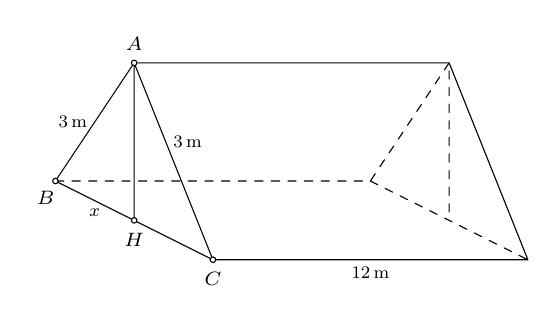
\begin{tikzpicture}[scale=1,>=stealth, font=\footnotesize, line join=round, line cap=round,declare function={h=2;d=4;}]
			\path
			(0,0) coordinate (B)
			(2,-1) coordinate (C)
			(barycentric cs:C=1,B=1)coordinate(H)
			(H)+(90:h) coordinate (A)
			(A)+(0:d)coordinate (D)
			(barycentric cs:A=-1,B=1,D=1)coordinate(E)
			(barycentric cs:A=-1,C=1,D=1)coordinate(F)
			(barycentric cs:A=-1,H=1,D=1)coordinate(K)
			;
			\draw[dashed] (B)--(E)--(D)--(K) (E)--(F);
			\draw (H)--(A)--(B)--(C)--(A)--(D)--(F)--(C);
			\foreach \x/\goc in {A/90,B/-120,C/-90,H/-90}
			\draw[fill=white] (\x) node[shift={(\goc:7pt)},font=\scriptsize]{$\x$} circle (1pt);
			\draw[draw=none] (C)--(F)node[below,midway,pos=0.5,scale=0.8]{$12\,\mathrm{m}$};
			\draw[draw=none] (C)--(A)node[right,midway,pos=0.6,scale=0.8]{$3\,\mathrm{m}$};
			\draw[draw=none] (B)--(A)node[left,midway,pos=0.5,scale=0.8]{$3\,\mathrm{m}$};
			\draw[draw=none] (B)--(H)node[below,midway,pos=0.5,scale=0.8]{$x$};
		\end{tikzpicture}
	\end{center}
	\loigiai{
		Đường cao hạ từ đỉnh lều xuống mặt đất bằng đoạn $AH$.\\
		Cửa lều $ABC$ là một tam giác cân tại đỉnh $A$, có các cạnh $AB=AC=3$ (m), $BC=x$.\\ Do đó, diện tích của tam giác $ABC$ bằng $S=\dfrac{1}{2}\cdot 3\cdot 3\cdot\sin A\leq\dfrac{9}{2}$ (m$^2$).\\
		Dấu bằng xảy ra khi và chỉ khi $\sin A=1\Leftrightarrow A=90^{\circ}$ hay $ABC$ trở thành tam giác vuông cân tại $A$, hai cạnh góc vuông không đổi bằng $3$ m, cạnh huyền bằng $x$.\\
		Khi đó, $x=BC=\sqrt{AB^{2}+AC^{2}}=\sqrt{3^{2}+3^{2}}=3\sqrt{2}\approx 4{,}24$ (m).\\ Suy ra đường cao $AH=\dfrac{BC}{2}\approx 2{,}12$ (m).\\
		Vậy đường cao từ đỉnh lều xuống mặt đất khoảng $2{,}12$ (m).
	}
\end{vd}
%%%=============================%%%

%%%=============VD_2=============%%%
\begin{vd}%[1H8V2-6]
	Một cột cờ bằng gỗ được chôn thẳng đứng trên mặt sân phẳng. Bạn Vinh đo từ một điểm trên mặt sân đến một điểm trên thân cột cờ là $1{,}5$ (m). Điểm trên thân cột cờ đó cách chân cột cờ là $1$ (m). Hãy giúp bạn Vinh tính xem điểm trên sân sẽ cách chân cột cờ bao nhiêu, biết rằng cột cờ luôn ở vị trí thẳng đứng so với mặt sân phẳng.
	\loigiai{
		\immini{Vì cột cờ luôn thẳng đứng vuông góc với mặt sân nên tam giác $ABC$ vuông tại $B$, có $AC=1{,}5$ (m); $BC=1$ (m).\\ Khi đó, $AB=\sqrt{AC^{2}-BC^{2}}=\sqrt{1{,}5^{2}-1^{2}}=\sqrt{1{,}25}\approx 1{,}12$ (m).\\
		Vậy điểm trên sân cách chân cột cờ khoảng $1{,}12$ (m).}
		{
			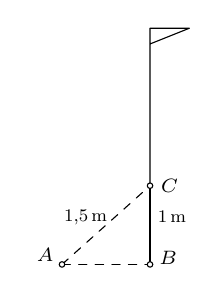
\begin{tikzpicture}[scale=1,>=stealth, font=\footnotesize, line join=round, line cap=round,declare function={d=sqrt(1.25);h=3;}]
				\path
				(0,0) coordinate (A)
				(d,0) coordinate (B)
				(B)+(90:1) coordinate (C)
				(B)+(90:h) coordinate (D)
				(D)+(0:0.5) coordinate (E)
				(B)+(90:h-0.2) coordinate (F)
				;
				\draw[dashed] (A)--(B);
				\draw[dashed] (A)--(C)node[left,midway,pos=0.6,scale=0.8]{$1{,}5\,\mathrm{m}$};
				\draw (C)--(D)--(E)--(F);
				\draw (B)--(C)node[right,midway,pos=0.6,scale=0.8]{$1\,\mathrm{m}$};
				\foreach \x/\goc in {A/150,B/20,C/0}
				\draw[fill=white] (\x) node[shift={(\goc:7pt)},font=\scriptsize]{$\x$} circle (1pt);
			\end{tikzpicture}
		}
	}
\end{vd}
%%%=============================%%%

%%%=============VD_3=============%%%
\begin{vd}%[1H8V2-6]
	Bạn Sơn mua một mô hình kim tự tháp Ai Cập thu nhỏ để tặng sinh nhật bạn. Mô hình này có đáy là hình vuông, cạnh đáy bằng $10$ cm, cạnh bên bằng nhau và có độ dài $10$ cm. Bạn Sơn muốn cho mô hình này vào một hộp quà hình hộp chữ nhật. Em hãy giúp bạn Sơn chọn hộp quà có chiều cao tối thiểu bao nhiêu để cho vừa kim tự tháp trên.
	\loigiai{
		\immini{
		Ta đi tính chiều cao của kim tự tháp, ký hiệu là $SO$.
		\\
		Đáy $ABCD$ của kim tự tháp là hình vuông cạnh $10$ cm, suy ra đường chéo $AC = 10\sqrt{2}$ cm.
		\\
		Xét tam giác $SAC$, ta có các cạnh $SA = 10$ cm, $SC = 10$ cm (theo giả thiết), và $AC = 10\sqrt{2}$ cm.
		\\
		Áp dụng định lí Pytago đảo, ta kiểm tra:
		\begin{itemize}
			\item $SA^2 + SC^2 = 10^2 + 10^2 = 100 + 100 = 200$.
			\item $AC^2 = (10\sqrt{2})^2 = 100 \cdot 2 = 200$.
		\end{itemize}
		Vì $SA^2 + SC^2 = AC^2$, nên tam giác $SAC$ vuông tại $S$.
		\\
		Kết hợp với $SA=SC$, ta có $\triangle SAC$ là tam giác vuông cân tại $S$.
		\\
		Chiều cao của kim tự tháp là $SO$, với $O$ là trung điểm của $AC$. Trong tam giác vuông $SAC$, $SO$ là đường trung tuyến ứng với cạnh huyền $AC$.
		\\
		Do đó, $SO = \dfrac{AC}{2} = \dfrac{10\sqrt{2}}{2} = 5\sqrt{2} \approx 7,1$ cm.
		\\
		Vậy chiều cao tối thiểu của hộp quà hình hộp chữ nhật là $7,1$ cm.}
		{
			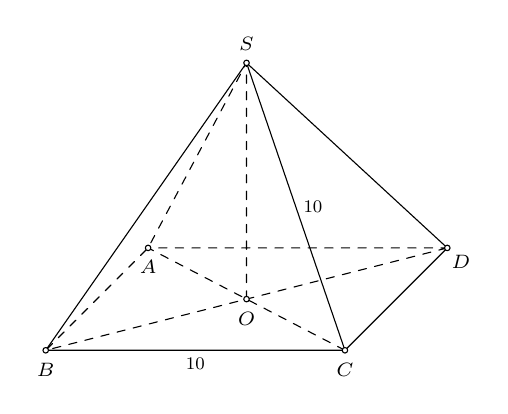
\begin{tikzpicture}[scale=1,>=stealth, font=\footnotesize, line join=round, line cap=round,declare function={h=3;}]
				\path
				(0,0) coordinate (A)
				(-1.3,-1.3) coordinate (B)
				(2.5,-1.3) coordinate (C)
				(barycentric cs:A=1,C=1,B=-1)coordinate(D)
				(barycentric cs:A=1,C=1)coordinate(O)
				(O)+(90:h) coordinate (S)
				;
				\draw[dashed] (O)--(S)--(A)--(B)--(D) (C)--(A)--(D);
				\draw (C)--(S)--(B)--(C)--(D)--(S);
				\foreach \x/\goc in {A/-90,B/-90,C/-90,D/-45,S/90,O/-90}
				\draw[fill=white] (\x) node[shift={(\goc:7pt)},font=\scriptsize]{$\x$} circle (1pt);
				\draw[draw=none] (C)--(B)node[below,midway,pos=0.5,scale=0.8]{$10$};
				\draw[draw=none] (C)--(S)node[right,midway,pos=0.5,scale=0.8]{$10$};
			\end{tikzpicture}
		}
	}
\end{vd}
%%%=============================%%%
\subsection{BÀI TẬP RÈN LUYỆN}
\ind{PHẦN I.} \inden{Câu trắc nghiệm nhiều phương án lựa chọn. Mỗi câu hỏi học sinh chỉ chọn một phương án.}\\
\setcounter{ex}{0}
\Opensolutionfile{ans}[ans/1H8-Bai2-TN]
%%%=============EX_1=============%%%
\begin{ex}%[1H8N2-2]
	[Trích đề thi GHKII - Trường THPT Ninh Bình - Bạc Liêu - Năm học: 2024-2025]
	Cho hình chóp $S.ABC$ có đáy $ABC$ là tam giác vuông tại $B$ và $SA\perp(ABC)$. Mệnh đề nào sau đây đúng?
	\choice
	{\True $BC\perp(SAB)$}
	{$AB\perp(SBC)$}
	{$AC\perp(SBC)$}
	{$AC\perp(SAB)$}
	\loigiai{
		\immini
		{
			Vì tam giác $ABC$ vuông tại $B$ nên ta có $AB\perp BC$.\\
			Hơn nữa $SA\perp(ABC)$, $BC\subset(ABC)$ nên $SA\perp BC$.\\
			Suy ra $BC\perp(SAB)$.
		}
		{
			\begin{tikzpicture}[declare function={goc=-45; a=3; b=0.45*a; h=3;}]
				\path 
				(0,0) coordinate (A)--+(0,h) coordinate (S)
				(a,0) coordinate (C)
				(goc:b) coordinate (B);
				\draw 
				pic[angle radius=3mm,draw] {right angle = S--A--B}
				pic[angle radius=3mm,draw] {right angle = A--B--C};
				\draw[dashed] (A)--(C);
				\draw (S)--(B) (S)--(A)--(B)--(C)--cycle;
				\foreach \x/\goc in {S/90,A/240,C/-60,B/-90}
				\draw[fill=white] (\x) node[shift={(\goc:7pt)},font=\scriptsize]{$\x$} circle (1pt);
			\end{tikzpicture}
		}
	}
\end{ex}
%%%=============================%%%

%%%=============EX_2=============%%%
\begin{ex}%[1H8N2-2]
	[Trích đề thi HKII - Trường THPT Lý Thái Tổ - Bắc Ninh - Năm học: 2024-2025]
	Cho hình chóp $S.ABC$ có đáy $ABC$ là tam giác cân tại $B$. Cạnh $SA$ vuông góc với mặt phẳng đáy và gọi $M$ là trung điểm cạnh $AC$. Đường thẳng $BM$ vuông góc với mặt phẳng nào dưới đây?
	\choice
	{\True $(SAC)$}
	{$(SBC)$}
	{$(SAB)$}
	{$(ABC)$}
	\loigiai
	{
		\immini
		{
			Ta có $\heva{& BM\perp AC\\& BM\perp SA}\Rightarrow BM\perp(SAC)$.
		}
		{
			\begin{tikzpicture}[declare function={goc=-45; a=3; b=0.45*a; h=3;}]
			\path 
			(0,0) coordinate (A)--+(0,h) coordinate (S)
			(a,0) coordinate (C)
			(goc:b) coordinate (B)
			($(A)!0.5!(C)$) coordinate (M);
			\draw 
			pic[angle radius=2mm,draw] {right angle = S--A--B}
			pic[angle radius=2mm,draw] {right angle = A--B--C};
			\draw[dashed] (A)--(C) (B)--(M);
			\draw (S)--(B) (S)--(A)--(B)--(C)--cycle;
			\foreach \x/\goc in {S/90,A/240,C/-60,B/-90,M/90}
			\draw[fill=white] (\x) node[shift={(\goc:7pt)},font=\scriptsize]{$\x$} circle (1pt);
			\end{tikzpicture}
		}
	}
\end{ex}
%%%=============================%%%

%%%=============EX_3=============%%%
\begin{ex}%[Dự án đề kiểm tra Toán 11 GHKII NH24-25- Nguyễn Tấn Tài]%[THPT An Lương Đông - Huế]%[1H8N2-2]
	[Trích đề thi GHKII - Trường THPT An Lương Đông - Huế - Năm học: 2024-2025]
		Cho hình chóp $S.ABC$ có đáy là tam giác vuông tại $B$, $SA$ vuông góc với đáy. Đường thẳng $BC$ vuông góc với mặt phẳng nào sau đây?
		\choice
		{$(SAC)$}
		{$(SBC)$}
		{$(ABC)$}
		{\True $(SAB)$}
	\loigiai{
		\immini{Ta có\\
		$\heva{
			& AB\perp BC\quad(\triangle ABC\text{ là tam giác vuông tại B} )\\
			& SA\perp BC\quad(SA\perp(ABC)).
		}$\\
		Suy ra $BC\perp(SAB)$.}
		{\begin{tikzpicture}[declare function={goc=-45; a=3; b=0.45*a; h=3;}]
				\path 
				(0,0) coordinate (A)--+(0,h) coordinate (S)
				(a,0) coordinate (C)
				(goc:b) coordinate (B)
				;
				\draw 
				pic[angle radius=2mm,draw] {right angle = S--A--B}
				pic[angle radius=2mm,draw] {right angle = A--B--C};
				\draw[dashed] (A)--(C);
				\draw (S)--(B) (S)--(A)--(B)--(C)--cycle;
				\foreach \x/\goc in {S/90,A/240,C/-60,B/-90}
				\draw[fill=white] (\x) node[shift={(\goc:7pt)},font=\scriptsize]{$\x$} circle (1pt);
		\end{tikzpicture}}
	}
\end{ex}
%%%=============================%%%

%%%=============EX_4=============%%%
\begin{ex}%[1H8N2-3]%[Lớp 11 - Học kì II - THPT XUYÊN MỘC - BÀ RỊA VŨNG TÀU]%[Võ Thị Thùy Trang]
	[Trích đề thi HKII - Trường THPT Xuyên Mộc - Bà Rịa Vũng Tàu - Năm học: 2024-2025]
	Cho hình chóp $S.ABCD$ có $SA\perp(ABCD)$, tứ giác $ABCD$ là hình chữ nhật. Tìm khẳng định \textbf{sai}.
	\choice
	{$SA\perp AB$}
	{$BD\perp SA$}
	{\True $AC\perp BD$}
	{$AB\perp BC$}
	\loigiai{
		Ta có $ABCD$ là hình chữ nhật nên $AC\perp BD$ là sai.}
\end{ex}
%%%=============================%%%

%%%=============EX_5=============%%%
\begin{ex}%[1H8N2-1]
	[Trích đề thi GHKII - Trường THPT Trần Cao Vân - Khánh Hoà - Năm học: 2024-2025]
	Trong không gian, mệnh đề nào sau đây đúng?
	\choice
	{Hai đường thẳng không cắt nhau và không song song thì chéo nhau}
	{Hai mặt phẳng phân biệt cùng vuông góc với một mặt phẳng thì song song với nhau}
	{\True Hai đường thẳng phân biệt cùng vuông góc với một mặt phẳng thì song song với nhau}
	{Hai đường thẳng phân biệt cùng vuông góc với một đường thẳng thì song song với nhau}
	\loigiai{
		Hai đường thẳng phân biệt cùng vuông góc với một mặt phẳng thì song song với nhau
	}
\end{ex}
%%%=============================%%%

%%%=============EX_6=============%%%
\begin{ex}%[1H8N2-1]
	Trong không gian cho điểm $O$ và đường thẳng $d$. Qua điểm $O$ có bao nhiêu mặt phẳng vuông góc với đường thẳng $d$?
	\choice
	{$2$}
	{\True $1$}
	{Vô số}
	{$3$}
	\loigiai{
		Theo tính chất $1$: Có duy nhất một mặt phẳng đi qua một điểm cho trước và vuông góc với một đường thẳng cho trước.
	}
\end{ex}
%%%=============================%%%

%%%=============EX_7=============%%%
\begin{ex}%[1H8N2-1]
	[Trích đề thi GHKII - Trường THPT Edison - Hải Phòng - Năm học: 2024-2025]
	Trong không gian, cho đường thẳng $\Delta$ không nằm trong mặt phẳng $(P)$. Khi nào đường thẳng $\Delta$ vuông góc với mặt phẳng $(P)$?
	\choice
	{Vuông góc với một đường thẳng $a$ mà $a$ song song với $(P)$}
	{Vuông góc với mọi đường thẳng nằm trong $(P)$}
	{\True Vuông góc với hai đường thẳng phân biệt nằm trong $(P)$}
	{Vuông góc với đường thẳng $a$ nằm trong $(P)$}
	\loigiai{
		Một đường thẳng được gọi là vuông góc với một mặt phẳng khi nó vuông góc với mọi đường thẳng nằm trong mặt phẳng đó.\\
		Điều này có nghĩa là nếu đường thẳng $\Delta$ vuông góc với hai đường thẳng phân biệt nằm trong mặt phẳng $(P)$ mà không song song với nhau, thì $(\Delta)$ cũng vuông góc với mặt phẳng.
	}
\end{ex}
%%%=============================%%%

%%%=============EX_8=============%%%
\begin{ex}%[1H8N2-5]
	[Trích đề thi GHKII - Trường THPT Trần Cao Vân - Khánh Hoà - Năm học: 2024-2025]
	Cho hình chóp $S.ABCD$ có đáy $ABCD$ là hình thoi tâm $O$, $SO$ vuông góc với đáy (hình vẽ). Hình chiếu của điểm $B$ trên mặt phẳng $(SAC)$ là
		\choice
		{Điểm $C$}
		{Điểm $S$}
		{\True Điểm $O$}
		{Điểm $A$}
	\loigiai{
		\immini{Ta có $\heva{&BO\perp SO\subset(SAC)\\& BO\perp AC\subset(SAC)\\& SO\cap AC=O.}$\\
		Suy ra $BO\perp(SAC)$ tại $O$.\\
		Vậy $O$ là hình chiếu của $B$ trên mặt phẳng $(SAC)$.
		}
		{	
		\begin{tikzpicture}[font=\scriptsize]
				\tikzset{declare function={a=3.5; b=2; h=3;}}
				\path (0,0) coordinate (A)
				(a,0) coordinate (D)
				(-135:b) coordinate (B)
				($(B)+(D)$) coordinate (C)
				($(A)!0.5!(C)$) coordinate (O)
				($(O)+(0,h)$) coordinate (S);
				\path pic[draw,angle radius=6pt]{right angle=A--O--S};
				\path pic[draw,angle radius=6pt]{right angle=D--O--S};
				\draw[dashed] (B)--(A)--(D)--cycle (C)--(A)--(S)--(O);
				\draw (S)--(B)--(C)--(D)--cycle (S)--(C);
				\foreach \t/\g in {A/150,B/-90,C/-60,D/60,S/90,O/-90}{
					\draw[fill=white] (\t) circle (1pt) node[shift={(\g:7pt)},font=\scriptsize]{$\t$};
				}
		\end{tikzpicture}
		}
	}
\end{ex}
%%%=============================%%%

%%%=============EX_9=============%%%
\begin{ex}%[1H8H2-5]
	\immini{Một cây dù đồng tâm được đặt theo phương thẳng đứng so với mặt đất. Vào thời điểm $12$ giờ trưa, ánh nắng mặt trời chiếu vuông góc xuống mặt đất ta thấy bóng của tán dù là một hình lục giác đều có cạnh là $0{,}5$ m. Biết rằng khoảng cách từ đỉnh dù đến một đỉnh bất kỳ của lục giác đều trên mặt đất là $2{,}5$ m. Giả sử chiều cao của đế dù là không đáng kể, khi đó chiều cao của thân dù là bao nhiêu mét?(Thân dù được xác định từ đỉnh dù đến mặt đất).
		\choice
		{\True $2{,}45$ m}
		{$2{,}25$ m}
		{$2{,}15$ m}
		{$2{,}35$ m}
	}{
		\definecolor{cadmiumgreen}{rgb}{0.0, 0.42, 0.24}
		\definecolor{tumbleweed}{rgb}{0.87, 0.67, 0.53}%màu cát
		\begin{tikzpicture}[line join=round, line cap=round,scale=0.8,transform shape]
			\clip (-4,-4) rectangle (4,4);
			\tikzset{du/.pic={
					\draw[tumbleweed,line width=4,opacity=0.75] (1.65,1.8)--(-.1,2.1)--(1.1,.85)%C,B
					(-.65,.7)--(-.1,2.1)--(-1.85,1.5) %A,F
					(-1.4,2.52)--(-.1,2.1)--(.45,2.7) %E,D
					(-.1,2.1)--(-.1,-1.5)
					(-1.1,1.75)--(-.1,1.7)--(.8,1.92)
					(-.8,2.3)--(-.1,1.7)--(.2,2.37)
					(-.45,1.2)--(-.1,1.7)--(.65,1.3)
					;
					\def\H{
						(-1.3,2.5)
						..controls +(-5:.2) and +(-165:0.15) .. (.4,2.65)
						..controls +(-50:.1) and +(140:.1) .. (1.6,1.8)
						..controls +(-140:.06) and +(80:0.27) .. (1.1,.9)--(-.6,.75)
						..controls +(120:.1) and +(-30:0.2) .. (-1.8,1.55)
						..controls +(50:.1) and +(-115:0.2) .. cycle
						;}
					\draw \H;
					\fill[cadmiumgreen!80,opacity=0.75] \H;
			}}
			\path
			(-.1,-1.5) coordinate (H)
			($(H)+(60:1.2)$) coordinate (D)
			($(D)+(-1.5,-.3)$) coordinate (E)
			($(H)+(0:1.2)$) coordinate (C)
			($(H)+(200:1.3)$) coordinate (F)
			($(H)+(-50:1.2)$) coordinate (B)
			($(B)+(-1.2,-.3)$) coordinate (A)
			(-.1,2.1)coordinate (G);
			\draw[fill=black] ($(H)+(.35,-.07)$) arc(0:360:.35 and .2);
			\draw[fill=gray] ($(H)+(.36,0)$) arc(0:360:.36 and .2);
			\path (0,0)pic[scale=1]{du};
	\end{tikzpicture}}
	\loigiai{
		\immini{Giả sử bóng của tán dù là hình lục giác đều $ABCDEF$ như hình vẽ minh họa.\\
			Vì dù được đặt theo phương thẳng đứng so với mặt đất nên ta có thân dù vuông góc với mặt đất cũng như vuông góc với mặt phẳng $\left(ABCDEF\right)$.\\
			Tức là, ta có $GH\perp\left(ABCDEF\right)$ mà $AH\subset\left(ABCDEF\right)$ nên $GH\perp AH$.\\
			Theo tính chất của lục giác đều, ta có $AH=0{,}5$ m.\\
			Xét tam giác $AHG$ vuông tại $H$ ta có $$GH=\sqrt{AG^2-AH^2}=\sqrt{2{,}5^2-0{,}5^2}=\sqrt{6}\approx 2{,}45\text{m}.$$
			Vậy chiều cao của thân dù là khoảng $2{,}45$ m.}{\definecolor{cadmiumgreen}{rgb}{0.0, 0.42, 0.24}
			\definecolor{tumbleweed}{rgb}{0.87, 0.67, 0.53}%màu cát
			\begin{tikzpicture}[line join=round, line cap=round,scale=0.8,transform shape]
				\clip (-4,-4) rectangle (4,4);
				\tikzset{du/.pic={
						\draw[tumbleweed,line width=4,opacity=0.75] (1.65,1.8)--(-.1,2.1)--(1.1,.85)%C,B
						(-.65,.7)--(-.1,2.1)--(-1.85,1.5) %A,F
						(-1.4,2.52)--(-.1,2.1)--(.45,2.7) %E,D
						(-.1,2.1)--(-.1,-1.5)
						(-1.1,1.75)--(-.1,1.7)--(.8,1.92)
						(-.8,2.3)--(-.1,1.7)--(.2,2.37)
						(-.45,1.2)--(-.1,1.7)--(.65,1.3)
						;
						\def\H{
							(-1.3,2.5)
							..controls +(-5:.2) and +(-165:0.15) .. (.4,2.65)
							..controls +(-50:.1) and +(140:.1) .. (1.6,1.8)
							..controls +(-140:.06) and +(80:0.27) .. (1.1,.9)--(-.6,.75)
							..controls +(120:.1) and +(-30:0.2) .. (-1.8,1.55)
							..controls +(50:.1) and +(-115:0.2) .. cycle
							;}
						\draw \H;
						\fill[cadmiumgreen!80,opacity=0.75] \H;
				}}
				\path
				(-.1,-1.5) coordinate (H)
				($(H)+(60:1.2)$) coordinate (D)
				($(D)+(-1.5,-.3)$) coordinate (E)
				($(H)+(0:1.2)$) coordinate (C)
				($(H)+(200:1.3)$) coordinate (F)
				($(H)+(-50:1.2)$) coordinate (B)
				($(B)+(-1.2,-.3)$) coordinate (A)
				(-.1,2.1)coordinate (G)
				;
				\draw[fill=black] ($(H)+(.35,-.07)$) arc(0:360:.35 and .2);
				\draw[fill=gray] ($(H)+(.36,0)$) arc(0:360:.36 and .2);
				\path (0,0)pic[scale=1]{du}
				;
				\foreach \x/\g in {H/45,A/-90,B/0,C/0,D/90,E/90,F/180,G/90}\draw[fill=black] (\x) circle (.05) +(\g:.3) node{$\x$};
				\draw[cadmiumgreen,line width=1.5,dashed] (F)--(E)--(D)--(C)--(B)--(A)--cycle (G)--(A);
		\end{tikzpicture}}
	}
\end{ex}
%%%=============================%%%

%%%=============EX_10=============%%%
\begin{ex}%[1H8H2-2]
	[Trích đề thi GHKII - Trường THPT Hoà Hội - Bà Rịa Vũng Tàu - Năm học: 2024-2025]
	Cho hình hộp $ABCD.A'B'C'D'$, có $AA'\perp(ABCD)$. Khẳng định nào sau đây là đúng?
	\choice
	{$AB\perp\left(AA'D'D\right)$}
	{$AC'\perp\left(A'B'C'D'\right)$}
	{\True $CC'\perp\left(A'B'C'D'\right)$}
	{$DC\perp\left(BB'C'C\right)$}
	\loigiai{
		\immini{
			Ta có $AA'\perp(ABCD)$ suy ra $AA'\perp(A'B'C'D')$.\\
			Mà $CC'\parallel AA'$, do đó $CC'\perp(A'B'C'D')$.
		}{
			\begin{tikzpicture}[declare function={a=3; b=0.45*a; h=0.65*a;}]
				\path (0:0) coordinate (A)
				(220:b) coordinate (B)
				($(B)+(a,0)$) coordinate (C)
				(a,0) coordinate (D)
				\foreach \x in {A,B,C,D}{(\x)++(90:h) coordinate (\x1)};
				\draw[dashed] (A1)--(A)--(B) (A)--(D);
				\draw (B1)--(A1)--(D1)--(C1) (D1)--(D)--(C) (B)--(C)--(C1)--(B1)--cycle;
				\foreach \x/\goc/\t in {A/45/A,B/-90/B,C/-90/C,D/0/D,A1/90/A',B1/90/B',C1/90/C',D1/90/D'}
				\draw[fill=white] (\x) circle (1pt) node[shift={(\goc:7pt)},font=\scriptsize]{$\t$};
			\end{tikzpicture}
		}
	}
\end{ex}
%%%=============================%%%

%%%=============EX_11=============%%%
\begin{ex}%[1H8H2-2]
	Cho lăng trụ $ABC.A'B'C'$ có $AA'\perp AB,AA'\perp AC$. Gọi $M$ là trung điểm của cạnh $BC$. Khẳng định nào dưới đây \textbf{sai}?
		\choice
		{$AA'\perp(ABC)$}
		{$AA'\perp(A'B'C')$}
		{$AM\perp AA'$}
		{\True $AM\perp(BCC'B')$}
	\loigiai{
		\immini{Ta có
		\begin{itemize}
			\item $AA'\perp AB,AA'\perp AC$ nên $AA'\perp(ABC)$.
			\item $AA'\perp(ABC)$ và $(ABC)\parallel(A'B'C')$ nên $AA'\perp(A'B'C')$.
			\item $AA'\perp(ABC)$ và $AM\subset(ABC)$ nên $AA'\perp AM$ hay $AM\perp AA'$.
		\end{itemize}
		Chưa đủ điều kiện để kết luận $AM\perp BC$ nên $AM\perp(BCC'B')$ sai.}
		{
		\begin{tikzpicture}[declare function={a=3.5; b=0.55*a; h=0.9*a;}]
				\path (0:0) coordinate (A)
				(-43:b) coordinate (B)
				(a,0) coordinate (C)
				\foreach \x in {A,B,C}{(\x)++(90:h) coordinate (\x1)}
				($(B)!0.5!(C)$) coordinate (M);
				\draw[dashed] (A)--(C) (A)--(M);
				\draw (B1)--(A1)--(C1)--cycle
				(A1)--(A)--(B)--(B1)
				(C1)--(C)--(B);
				\foreach \x/\goc/\t in {A/180/A,B/-90/B,C/0/C,A1/100/A',B1/85/B',C1/80/C',M/0/M}
				\draw[fill=white] (\x) circle (1pt) node[shift={(\goc:9pt)},font=\scriptsize]{$\t$};
		\end{tikzpicture}
		}
	}
\end{ex}
%%%=============================%%%

%%%=============EX_12=============%%%
\begin{ex}%[1H8H2-2]%[Đề thi HKII LỚP 11 THPT-TranPhu-TPHCM-NH24-25]
	[Trích đề thi HKII - Trường THPT Trần Phú - TP.HCM - Năm học: 2024-2025]
		Cho tứ diện $ABCD$ có $AB$, $AC$, $AD$ đôi một vuông góc nhau. Chọn khẳng định \textbf{sai} trong các khẳng định sau
		\choice
		{$AC\perp(ABD)$}
		{$AB\perp CD$}
		{$AC\perp BD$}
		{\True $AC\perp(BCD)$}
	\loigiai{
		\immini{Ta có $AC\perp AB$, $AC\perp AD$ nên $AC\perp(ABD)$. Suy ra $AC\perp BD$. \\
		Ta cũng có $AB\perp AC$, $AB\perp AD$ nên $AB\perp(ACD)$. Suy ra $AB\perp CD$. \\
		Vậy khẳng định \textbf{sai} là $AC\perp(BCD)$.}
		{\begin{tikzpicture}[scale=0.7, font=\footnotesize,line join=round, line cap=round, >=stealth]
				\path
				(0,0) coordinate (A)
				++(-120:2) coordinate (C)
				(3,0) coordinate (D)
				(0,3) coordinate (B)
				;
				\draw (C)--(D)--(B)--cycle;
				\draw[dashed] (A)--(C) (D)--(A)--(B);
				\pic[draw, angle radius=2mm]{right angle=D--A--C}
				pic[draw, angle radius=2mm]{right angle=D--A--A}
				;
				\foreach \x/\goc/\t in {C/180/C,D/-90/D,B/90/B,A/160/A}
				\draw[fill=white] (\x) circle (1pt) node[shift={(\goc:9pt)},font=\scriptsize]{$\t$};
		\end{tikzpicture}}
	}
\end{ex}
%%%=============================%%%

%%%=============EX_13=============%%%
\begin{ex}%[1H8H2-2]
	[Trích đề thi GHKII - Trường THPT Phan Đình Phùng - Hà Nội - Năm học: 2024-2025]
	Cho hình chóp $S.ABC$ có đáy là tam giác vuông tại $A$ và $SA\perp(ABC)$ (tham khảo hình vẽ bên dưới). Mệnh đề nào sau đây là đúng?
		\choice[2]
		{$BC\perp(SAB)$}
		{$AB\perp(SBC)$}
		{$BC\perp(SAC)$}
		{\True $AB\perp(SAC)$}
	\loigiai{
		\immini{Vì $\heva{&SA\perp(ABC)\\&AB\subset(ABC)}$ nên $SA\perp AB$. \hfill (1)\\
		Tam giác $ABC$ vuông tại $A$ nên $AB\perp AC$.\hfill (2)\\
		Từ (1) và (2) suy ra $AB\perp(SAC)$.}
		{	\begin{tikzpicture}[declare function={a=3; b=0.45*a; h=0.65*a;}]
				\path (0,0) coordinate (A)
				(a,0) coordinate (C)
				(-45:b) coordinate (B)
				($(A)+(0,h)$) coordinate (S);
				\foreach \x/\y/\z in {B/A/S,C/A/S}{
					\path pic[draw,angle radius=5pt]{right angle=\x--\y--\z};
				}
				\draw[dashed] (A)--(C);
				\draw (S)--(B) (S)--(A)--(B)--(C)--cycle;
				\foreach \x/\goc in {S/90,A/190,B/-90,C/0}
				\draw[fill=white] (\x) node[shift={(\goc:7pt)},font=\scriptsize]{$\x$} circle (1pt);
			\end{tikzpicture}}
	}
\end{ex}
%%%=============================%%%

%%%=============EX_14=============%%%
\begin{ex}%[1H8H2-1]
	[Trích đề thi HKII - Sở GD\&ĐT Nam Định - Năm học: 2024-2025]
	Trong không gian cho các đường thẳng $a$, $b$ và mặt phẳng $(P)$. Mệnh đề nào sau đây đúng?
	\choice
	{ Nếu $a$ vuông góc với hai đường thẳng phân biệt trong mặt phẳng $(P)$ thì $a\perp(P)$}
	{ Nếu $a\parallel(P)$ và $b\perp a$ thì $b\perp(P)$}
	{ Nếu $a\parallel(P)$ và $b\parallel a$ thì $b\parallel(P)$}
	{ \True Nếu $a\parallel(P)$ và $b\perp(P)$ thì $b\perp a$}
	\loigiai{
		Xét các mệnh đề
		\begin{itemize}
			\item {Nếu $a\parallel(P)$ và $b\parallel a$ thì $b\parallel(P)$:} Sai, vì $b$ có thể song song với $(P)$ hoặc $b$ có thể nằm trong $(P)$.
			\item {Nếu $a$ vuông góc với hai đường thẳng phân biệt trong $(P)$ thì $a\perp(P)$:} Sai, vì thiếu điều kiện hai đường thẳng đó phải \textbf{cắt nhau}.
			\item {Nếu $a\parallel(P)$ và $b\perp a$ thì $b\perp(P)$:} Sai, vì $b$ có thể là một đường thẳng nằm trong $(P)$ (hoặc song song với $(P)$) mà vẫn vuông góc với $a$.
			\item {Nếu $a\parallel(P)$ và $b\perp(P)$ thì $b\perp a$:} Đúng. Đây là tính chất theo định lý.
			\begin{itemize}
				\item Vì $a\parallel(P)$, tồn tại đường thẳng $a'\subset(P)$ sao cho $a'\parallel a$.
				\item Vì $b\perp(P)$, suy ra $b$ vuông góc với mọi đường thẳng trong $(P)$, do đó $b\perp a'$.
				\item Từ $b\perp a'$ và $a'\parallel a$, suy ra $b\perp a$.
			\end{itemize}
		\end{itemize}
	}
\end{ex}
%%%=============================%%%

%%%=============EX_15=============%%%
\begin{ex}%[1H8H2-3]
	[Trích đề thi HKII - Trường THPT Hướng Hóa - Quảng Trị - Năm học: 2024-2025]
	Cho hình lập phương $ABCD.A'B'C'D'$. Đường thẳng nào sau đây vuông góc với đường thẳng $BC$?
	\choice
	{$BC'$}
	{\True $A'B'$}
	{$BD'$}
	{$AD'$}
	\loigiai{
		\immini{Ta có $\heva{&AB\parallel A'B'\\&AB\perp BC}\Rightarrow A'B'\perp BC$.}
		{
			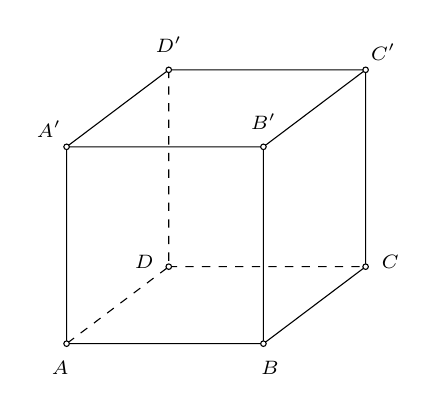
\begin{tikzpicture}[declare function={r=2.5;},font=\scriptsize]
				\path (0:0) coordinate (A)
				(0:r) coordinate (B)
				++(37:{0.65*r}) coordinate (C)
				++(180:r) coordinate (D)
				\foreach \x in {A,B,C,D}{(\x)++(90:r) coordinate (\x_1)};
				\draw[dashed] (D_1)--(D)--(A) (D)--(C);
				\draw (A)--(B)--(C) (A)--(A_1) (B)--(B_1) (C)--(C_1)(A_1)--(B_1)--(C_1)--(D_1)--cycle;
				\foreach \x/\goc/\t in {A/255/A, B/-75/B, C/10/C, D/170/D, A_1/135/A', B_1/90/B',
					C_1/45/C', D_1/90/D'}{
					\draw[fill=white] (\x) circle (1pt) node[shift={(\goc:9pt)}]{$\t$};
				}
			\end{tikzpicture}
	}
	}
\end{ex}
%%%=============================%%%

%%%=============EX_16=============%%%
\begin{ex}%[1H8H2-3]
	[Trích đề thi HKII - Trường THPT Trần Phú - TP.HCM - Năm học: 2024-2025]
	Cho tứ diện $ABCD$ có $AB=AC=2$, $DB=DC=3$. Khẳng định nào sau đây đúng?
	\choice
	{$DC\perp(ABC)$}
	{$AB\perp(BCD)$}
	{\True $BC\perp AD$}
	{$AC\perp BD$}
	\loigiai{
		\immini{Ta có $\triangle ABC$, $\triangle DBC$ lần lượt cân tại $A$, $D$.\\
			Gọi $H$ là trung điểm của $BC$.\\
			Suy ra $\heva{&AH\perp BC\\&DH\perp BC}\Rightarrow\heva{&AD\subset(ADH)\\&BC\perp(ADH)}\Rightarrow BC\perp AD$.}
		{\begin{tikzpicture}[declare function={a=4;},font=\scriptsize]
				\path	(0:0) coordinate (B)
				++(0:a) coordinate (D)
				++(-120:a/2) coordinate (C)
				($(B)+(70:a*0.8)$) coordinate (A)
				($(B)!0.5!(C)$) coordinate (H);
				\draw[dashed,smooth] (B)--(D)--(H);
				\draw[smooth] (B)--(A)--(D) (H)--(A)--(C)(B)--(C)--(D);
				\draw pic[draw, angle radius=0.2cm]{right angle=A--H--B};
				\draw pic[draw, angle radius=0.2cm]{right angle=C--H--D};
				\foreach \x/\goc in {A/90,B/180,C/-45,D/0,H/210}{
					\draw[fill=white] (\x) circle (1pt) node[shift={(\goc:9pt)}]{$\x$};
				}
		\end{tikzpicture}}
	}
\end{ex}
%%%=============================%%%

%%%=============EX_17=============%%%
\begin{ex}%[1H8H2-3]
	Cho hình chóp $S.ABC$ đáy $ABC$ là tam giác đều, cạnh bên $SA$ vuông góc với đáy. Gọi $M$, $N$ lần lượt là trung điểm của $AB$ và $SB$. Trong các mệnh đề sau, mệnh đề nào là mệnh đề {\bf sai}?
	\choice
	{$CM\perp SB$}
	{$CM\perp AN$}
	{\True $AN\perp BC$}
	{$MN\perp MC$}
	\loigiai{
		\immini{Ta có $\heva{&CM\perp AB\\&CM\perp SA\\&SA,\,AB\subset(SAB)}\Rightarrow CM\perp(SAB)\Rightarrow CM\perp SB$.\\
			Mà $AN\subset(SAB)\Rightarrow CM\perp AN$.\\
			Mặt khác $\heva{&MN\parallel SA\\&SA\perp(ABC)}\Rightarrow MN\perp(ABC)$.\\
			Vì $\heva{&MN\perp(ABC)\\&CM\subset(ABC)}\Rightarrow MN\perp CM$.}
		{\begin{tikzpicture}
				\def\a{4} %Khai báo cạnh
				\def\h{3}
				\path	(0:0) coordinate (A)
				++(0:\a) coordinate (B)
				++(-150:4*\a/5) coordinate (C)
				($(A)+(90:\h)$) coordinate (S)
				($(A)!0.5!(B)$) coordinate (M)
				($(S)!0.5!(B)$) coordinate (N);
				\draw[smooth] (A)--(C)--(B) (A)--(S) (B)--(S) (C)--(S);
				\draw[dashed,smooth](N)--(A)--(B) (M)--(C) (M)--(N);
				\foreach \x/\goc in {A/180,B/0,C/-135,S/90,M/-60,N/30}{
					\draw[fill=white] (\x) circle (1pt) node[shift={(\goc:9pt)}]{$\x$};
				}
		\end{tikzpicture}}
	}
\end{ex}
%%%=============================%%%

%%%=============EX_18=============%%%
\begin{ex}%[1H8H2-4]
	[Trích đề thi GHKII - Trường THPT Nguyễn Huệ - Bà Rịa Vũng Tàu - Năm học: 2023-2024]
	Cho hình chóp $S.ABCD$ có đáy $ABCD$ là hình vuông và $SA\perp(ABCD)$. Gọi $(P)$ là mặt phẳng đi qua điểm $A$ và vuông góc với đường thẳng $SD$. Gọi $E$ là hình chiếu vuông góc của $A$ trên đường thẳng $SD$. Mặt phẳng $(P)$ là mặt phẳng nào?
	\choice
	{$(AKE)$ với $K$ là trung điểm của cạnh $BC$}
	{$(AEM)$ với $M$ là hình chiếu vuông góc của $A$ trên $SC$ }
	{\True $(ABE)$}
	{$(ACE)$}
	\loigiai{
		\immini{Mặt phẳng $(P)$ đi qua $A$ và vuông góc với $SD$ là $(ABE)$.}{
			\begin{tikzpicture}
				\tikzset{declare function={a=3; b=2; h=3;}}
				\path (0,0) coordinate (A)
				(a,0) coordinate (D)
				(-120:b) coordinate (B)
				($(B)+(D)$) coordinate (C)
				(0,h) coordinate (S)
				($(S)!(A)!(D)$) coordinate (E);
				\path pic[draw,angle radius=5pt]{right angle=B--A--S};
				\path pic[draw,angle radius=5pt]{right angle=D--A--S};
				\path pic[draw,angle radius=5pt]{right angle=A--E--S};
				\draw[dashed] (B)--(A)--(D) (A)--(S) (A)--(E)--(B);
				\draw (S)--(B)--(C)--(D)--cycle (S)--(C);
				\foreach \t/\g in {A/180,B/180,C/0,D/0,S/90,E/90}{
					\draw[fill=white] (\t) circle (1pt) node[shift={(\g:9pt)},font=\scriptsize]{$\t$};
				}
			\end{tikzpicture}
		}
	}
\end{ex}
%%%=============================%%%

%%%=============EX_19=============%%%
\begin{ex}%[1H8H2-2]
	[Trích đề thi HKII - Trường THPT Chuyên Trần Đại Nghĩa - TP.HCM - Năm  học: 2024-2025]
	\immini{Cho hình chóp tam giác $S.ABC$ có $SA\perp(ABC)$, tam giác $ABC$ vuông tại $B$. Gọi $H$ là hình chiếu của $A$ trên $SB$ (tham khảo hình vẽ). Xét các khẳng định sau
		\begin{enumerate}[(1)]
			\item $AH\perp SC$.
			\item $BC\perp(SAB)$.
			\item $SC\perp AB$.
		\end{enumerate}
		Có bao nhiêu khẳng định đúng?
		\choice
		{$1$}
		{$0$}
		{\True$2$}
		{$3$}}
	{\begin{tikzpicture}[scale=0.7, font=\footnotesize, line join=round, line cap=round, >=stealth]
			\path (0,0) coordinate(A)
			--+(1.5,-2)coordinate (B)
			--+(5,0) coordinate (C)
			--+(0,5) coordinate (S)
			(S)--(B)coordinate[pos=0.6](H);
			\draw (S)--(A)--(B)--(C)--(S)--cycle (S)--(B) (A)--(H);
			\draw[dashed] (A)--(C);
			\draw pic[draw, angle radius=0.2cm]{right angle=S--A--C};
			\draw pic[draw, angle radius=0.2cm]{right angle=A--B--C};
			\draw pic[draw, angle radius=0.2cm]{right angle=A--H--B};
			\foreach \t/\g in {A/180,B/-90,C/0,S/90,H/60}{
				\draw[fill=white] (\t) circle (1pt) node[shift={(\g:9pt)},font=\scriptsize]{$\t$};
			}
	\end{tikzpicture}}
	\loigiai{
		Ta phân tích từng khẳng định
		\begin{enumerate}
			\item $AH\perp SC$ đúng.\\
			$\heva{&BC\perp SA\\&BC\perp AB}\Rightarrow BC\perp(SAB)\Rightarrow BC\perp AH$.\\
			Mặt khác $AH\perp SB$ nên $AH\perp(SBC)$ mà $SC\subset(SBC)$ nên $AH\perp SC$.
			\item $BC\perp(SAB)$ đúng.\\
			Chứng minh trên.
			\item $SC\perp AB$ sai.\\
			Giả sử $SC\perp AB$. \\
			Ta có $\heva{&AB\perp SC\\&AB\perp SA}\Rightarrow AB\perp(SAC)\Rightarrow AB\perp AC$ (vô lý).
		\end{enumerate}
	}
\end{ex}
%%%=============================%%%

%%%=============EX_20=============%%%
\begin{ex}%[1H8H2-2]
	Cho hình chóp $S.ABC$ có $SA$ vuông góc với mặt phẳng $(ABC)$, $SA=2a$, tam giác $ABC$ vuông tại $B$, $AB=a\sqrt{3}$ và $BC=a$. Tính góc giữa hình chiếu của đường thẳng $SC$ xuống mặt phẳng $(SAB)$ và $AB$.
	\choice
	{\True $49{,}1^\circ$}
	{$49{,}3^\circ$}
	{$48{,}3^\circ$}
	{$50^\circ$}
	\loigiai{
		\immini{Ta có $BC\perp AB,BC\perp SA$ nên $BC\perp(SAB)$.\\
			Suy ra hình chiếu của $SC$ và mặt phẳng $(SAB)$ là $SB$.\\
			Khi đó $(SB,AB)=\widehat{SBA}$.\\
			Xét $\triangle SAB$ có $\tan\widehat{SBA}=\dfrac{SA}{AB}=\dfrac{2a}{a\sqrt{3}}\Rightarrow\widehat{SBA}\approx 49{,}1^\circ$.}
		{\begin{tikzpicture}
				\def\a{3}
				\path	(0:0) coordinate (A)
				(0:\a) coordinate (C)
				(-35:.8*\a) coordinate (B)
				($(A)+(90:\a)$) coordinate (S);
				\draw	(A)--(B)--(C)
				(A)--(S)	(B)--(S)	(C)--(S);
				\draw[dashed]	(A)--(C)	;
				\foreach \t/\g in {A/180,B/-45,C/0,S/90}{
					\draw[fill=white] (\t) circle (1pt) node[shift={(\g:9pt)},font=\scriptsize]{$\t$};
				}
				\draw pic[draw,angle radius=2mm]{right angle=C--A--S}
				pic[draw,angle radius=2mm]{right angle=A--B--C};
		\end{tikzpicture}}
	}
\end{ex}
%%%=============================%%%

\Closesolutionfile{ans}

\ind{PHẦN II.} \inden{Câu trắc nghiệm đúng sai. Trong mỗi ý a), b), c), d) ở mỗi câu, học sinh chọn đúng hoặc sai.}\\
\setcounter{ex}{0}
\Opensolutionfile{ans}[ans/1H8-Bai2-DS]

%%%=============EX_1=============%%%
\begin{ex}%[1H8H2-5]
	Cho tứ diện $OABC$ có $OA$, $OB$, $OC$ đôi một vuông góc với nhau. Gọi $H$ là hình chiếu của $O$ trên $(ABC)$.
	\choiceTF
	{\True $\dfrac{1}{OH^2}=\dfrac{1}{OA^2}+\dfrac{1}{OB^2}+\dfrac{1}{OC^2}$}
	{\True $H$ là trực tâm tam giác $ABC$}
	{$AH\perp(OBC)$}
	{\True $BC\perp(AOH)$}
	\loigiai{
		\immini{\begin{itemchoice}
				\itemch
				Gọi $I=AH\cap BC$.\\
				Tam giác vuông $AOI$, ta có $\dfrac{1}{OH^2}=\dfrac{1}{OA^2}+\dfrac{1}{OI^2}$.\\
				Tam giác vuông $BOC$, ta có $\dfrac{1}{OI^2}=\dfrac{1}{OB^2}+\dfrac{1}{OC^2}$.\\
				Từ đó suy ra $\dfrac{1}{OH^2}=\dfrac{1}{OA^2}+\dfrac{1}{OB^2}+\dfrac{1}{OC^2}$.
				\itemch
				Từ $BC\perp(AOH)\Rightarrow BC\perp AH$.\\
				Chứng minh tương tự ta có $AB\perp CH$.\\
				Vậy $H$ là trực tâm $\triangle ABC$.
				\itemch
				Giả sử $AH\perp(OBC)$. \\
				Theo chứng minh trên có $AO\perp(OBC)$. Suy ra $A$, $O$, $H$ thẳng hàng (vô lí).
				\itemch
				Ta có $\heva{& OA\perp OB\\
					& OA\perp OC\\
				}\Rightarrow OA\perp(OBC)\Rightarrow OA\perp BC$.\\
				Lại có $OH\perp\left(ABC\right)\Rightarrow OH\perp BC$.\\
				Từ hai điều trên, ta suy ra $BC\perp(AOH)$.
		\end{itemchoice}}
		{\begin{tikzpicture}[>=stealth,line join=round,line cap=round,font=\footnotesize,scale=1]
				\def\a{4}
				\def\b{3}
				\def\h{3}
				\path
				(0,0)coordinate (O)
				+(90:\h)coordinate (A)
				+ (0:\a)coordinate (C)
				+ (-30:\b)coordinate (B)
				($(B)!.4!(C)$)coordinate (I)
				($(A)!.4!(I)$)coordinate (H);
				\draw (A)--(O)--(B)--(C)--cycle (I)--(A)--(B);
				\draw[dashed] (O)--(C) (O)--(I) (O)--(H);
				\draw pic[draw,angle radius=2mm] {right angle = O--I--C}
				pic[draw,angle radius=2mm] {right angle = O--H--I};
				\foreach \t/\g in {A/90,O/180,B/-90,C/0,I/-20,H/0}{
					\draw[fill=white] (\t) circle (1pt) node[shift={(\g:9pt)},font=\scriptsize]{$\t$};
				}
			\end{tikzpicture}
		}
	}
\end{ex}
%%%=============================%%%

%%%=============EX_2=============%%%
\begin{ex}%[1H8H2-3]
	Cho hình chóp $S.ABCD$ có đáy là hình chữ nhật và $SA$ vuông góc với mặt phẳng đáy. Gọi $H$, $K$ theo thứ tự là hình chiếu của $A$ trên các cạnh $SB$, $SD$.
	\choiceTF
	{\True Tam giác $SCD$ vuông}
	{\True Tam giác $SBC$ vuông}
	{\True $SC\perp(AHK)$}
	{\True $HK\perp SC$}
	\loigiai{
		\immini{
			Do $SA\perp(ABCD)$ nên $SA\perp CB$ và $SA\perp CD$.\\
			Ta có
			\begin{itemchoice}
				\itemch Ta có $CD\perp SA$, $CD\perp AD$ ($ABCD$ là hình chữ nhật) nên $CD\perp(SAD)$, suy ra $CD\perp SD$.\\
				Do đó, tam giác $SCD$ vuông tại $D$.
				\itemch Ta có $CB\perp SA$, $CB\perp AB$ ($ABCD$ là hình chữ nhật) nên $CB\perp(SAB)$, suy ra $CB\perp SB$.\\
				Do đó, tam giác $SBC$ vuông tại $B$.
				\itemch Do $CB\perp(SAB)$ nên $CB\perp AH$ mà $AH\perp SB$ nên $AH\perp SC$.\\
				Do	 $CD\perp(SAD)$ nên $CD\perp AK$ mà $AK\perp SD$ nên $AK\perp SC$.\\
				Vậy $SC\perp(AHK)$.
				\itemch Do $SC\perp(AHK)$ nên $SC\perp HK$.
		\end{itemchoice}}
		{\begin{tikzpicture}[>=stealth,line join=round,line cap=round,font=\footnotesize,scale=1]
				\def\a{3}
				\def\b{1}
				\path (0,0)coordinate (O)
				+(140:\b)coordinate (A)
				(A)+(0:\a)coordinate (D) (A)+(90:\a)coordinate (S)
				($(A)!2!(O)$)coordinate (C)
				($(D)!2!(O)$)coordinate (B)
				($(S)!.6!(B)$)coordinate (H)
				($(S)!.4!(D)$)coordinate (K)
				;
				\draw (S)--(B)--(C)--(D)--cycle (S)--(C) ;
				\draw[dashed](S)--(A)--(D) (A)--(B) (H)--(A)--(K)--cycle;
				\foreach \t/\g in {S/90,A/-90,B/210,C/-30,D/0,H/180,K/60}{
					\draw[fill=white] (\t) circle (1pt) node[shift={(\g:9pt)},font=\scriptsize]{$\t$};
				}
				\draw pic[draw,angle radius=2mm] {right angle = S--K--A};
				\draw pic[draw,angle radius=2mm] {right angle = S--H--A};
		\end{tikzpicture}}
	}
\end{ex}
%%%=============================%%%

%%%=============EX_3=============%%%
\begin{ex}%[1H8H2-2]
	[Trích đề thi GHKII - Trường THPT Hoà Hội - Bà Rịa Vũng Tàu - Năm học: 2024-2025]
	Cho hình chóp $S. ABCD$ có đáy $ABCD$ là hình vuông và $SA$ vuông góc với $(ABCD)$.
	\choiceTF
	{\True $SA\perp BC$}
	{\True $CD\perp(SAD)$}
	{\True $BD\perp SC$}
	{Góc giữa hai đường thẳng $SB$ và $CD$ là $\widehat{SBD}$}
	\loigiai{
		\immini{
			\begin{itemchoice}
				\itemch Ta có $SA\perp(ABCD)$ nên $SA\perp BC$.
				\itemch Ta có $\heva{&CD\perp AD\\&CD\perp SA}$ suy ra $CD\perp(SAD)$.
				\itemch Do $ABCD$ là hình vuông nên $BD\perp AC$,\\
				lại có $SA\perp(ABCD)\Rightarrow BD\perp SA$.\\
				Do đó $BD\perp(SAC)\Rightarrow BD\perp SC$.
				\itemch Ta có $AB\parallel CD$ nên $(SB,CD)=(SB,AB)=\widehat{SBA}$.
			\end{itemchoice}
		}{
			\begin{tikzpicture}[>=stealth,smooth,line join=round,line cap=round,font=\footnotesize,scale=1]
				\path
				(0,0) coordinate (A)
				(-145:2) coordinate (B)
				(0:3) coordinate (D)
				($(D)-(A)+(B)$) coordinate (C)
				($(A)+(0,2.5)$) coordinate (S)
				;
				\draw[dashed] (S)--(A)--(B) (A)--(D)--(B) (A)--(C);
				\draw (B)--(C)--(D)--(S)--(B) (S)--(C);
				\foreach \t/\g in {A/140,S/90,B/-160,C/-40,D/0}{
					\draw[fill=white] (\t) circle (1pt) node[shift={(\g:9pt)},font=\scriptsize]{$\t$};
				}
			\end{tikzpicture}
		}
	}
\end{ex}
%%%=============================%%%

%%%=============EX_4=============%%%
\begin{ex}%[1H8V2-2]
	[Trích đề thi GHKII - Trường THPT Nguyễn Thượng Hiền - TP.HCM - Năm học: 2024-2025]
	Cho hình chóp $S.ABCD$ có đáy $ABCD$ là hình vuông. Gọi $I$, $H$ lần lượt là trung điểm của $AB$, $BC$. Biết rằng $SI\perp(ABCD)$.
	\choiceTF
	{\True $BC\perp(SAB)$}
	{$BD\perp(SIC)$}
	{\True $SI\perp AD$}
	{Góc giữa hai đường thẳng $DH$ và $SC$ bằng $45^{\circ}$}
	\loigiai{
		\begin{center}
			\begin{tikzpicture}[scale=1, font=\footnotesize,line join=round, line cap=round, >=stealth]
				\path
				(0,0) coordinate (A)
				++(-140:2) coordinate (B)
				++(0:3.5) coordinate (C)
				($(A)+(C)-(B)$) coordinate (D)
				($(A)!1/2!(B)$) coordinate (I)
				($(I)+(0,4)$) coordinate (S)
				($(B)!1/2!(C)$) coordinate (H)
				;
				\foreach \i in{B,C,D}{\draw (S)--(\i);};
				\draw (B)--(C)--(D);
				\draw[dashed] (S)--(A)--(B) (A)--(D)--(H) (S)--(I)--(C);
				\pic[draw,angle eccentricity=1.8,angle radius=2mm]{right angle=S--I--A};
				\foreach \t/\g in {A/45,B/-90,C/-90,D/-40,S/90,I/170,H/-90}{
					\draw[fill=white] (\t) circle (1pt) node[shift={(\g:9pt)},font=\scriptsize]{$\t$};
				}
			\end{tikzpicture}
			\begin{tikzpicture}[scale=0.8, font=\footnotesize,line join=round, line cap=round, >=stealth]
				\def\a{4} %%chiều dài
				\def\b{4} %%chiều rộng
				\path
				(0,0) coordinate (A)
				(\a,0) coordinate (D)
				(0,-\b) coordinate (B)
				($(B)+(D)-(A)$) coordinate (C)
				($(C)!1/2!(B)$) coordinate (H)
				($(A)!1/2!(B)$) coordinate (I)
				;
				\draw (A)--(D) (A)--(B) (B)--(C)--(D)--(H) (C)--(I)
				;
				\foreach \t/\g in {A/90,D/90,C/-90,B/-90,H/-90,I/180}{
					\draw[fill=white] (\t) circle (1pt) node[shift={(\g:9pt)},font=\scriptsize]{$\t$};
				}
			\end{tikzpicture}
		\end{center}
		\begin{itemchoice}
			\itemch Ta có $SI\perp(ABCD)$ suy ra $SI\perp BC$. \\
			Ta có $\heva{&BC\perp AB\\&BC\perp SI\\&\text{Trong}(SAB),AB\cap SI=I}\Rightarrow BC\perp(SAB)$.
			\itemch Giả sử $BD\perp(SIC)$. Khi đó $BD\perp IC$. Mà $BD\perp AC$ nên $IC\equiv AC$ (vô lý). \\
			Vậy $BD$ không vuông góc với $(SIC)$.
			\itemch Ta có $SI\perp(ABCD)$ suy ra $SI\perp AD$.
			\itemch Ta có $\triangle DCH=\triangle CBI$ (c-g-c). Suy ra $\widehat{CDH}=\widehat{BCI}$. \\
			Mà $\widehat{BCI}+\widehat{DCI}=\widehat{BCD}=90^{\circ}$ nên $\widehat{CDH}+\widehat{DCI}=90^{\circ}$. \\
			Do đó $DH\perp CI$. \\
			Ta có $SI\perp(ABCD)$, $DH\subset(ABCD)$ suy ra $SI\perp DH$. Mà $DH\perp CI$ nên $DH\perp(SIC)$. \\
			Do đó $DH\perp SC$. \\
			Vậy $(DH,SC)=90^{\circ}$.
		\end{itemchoice}
	}
\end{ex}
%%%=============================%%%

%%%=============EX_5=============%%%
\begin{ex}%[1H8V2-3]
	Cho hình chóp $S. ABC$ có $SA\perp(ABC)$ và tam giác $ABC$ vuông tại $B$. Gọi $H$, $K$ là hình chiếu vuông góc của $A$ trên các cạnh $SB$, $SC$. Xét tính đúng sai của các mệnh đề sau.
	\choiceTF
	{Tam giác $SBC$ cân tại $B$}
	{\True $AH$ vuông góc với mặt phẳng $(SBC)$}
	{\True $(SC,HK)=90^{\circ}$}
	{\True Giả sử $HK$ cắt $BC$ tại $D$. Khi đó, $(AC,AD)=90^{\circ}$}
	\loigiai{
		\immini{
			\begin{itemchoice}
				\itemch Ta có $\heva{
					&BC\perp AB\\
					&BC\perp SA(\text{do~}SA\perp(ABC))
				}$ $\Rightarrow$ $BC\perp(SAB)$.\\
				Mà $SB\subset(SAB)$ nên $BC\perp SB$ hay tam giác $SBC$ vuông tại $B$.
				\itemch Ta có $\heva{
					&AH\perp SB\\
					&AH\perp BC(\text{do~}BC\perp(SAB))
				}$ $\Rightarrow$ $AH\perp(SBC)$.
				\itemch Ta có $\heva{
					&SC\perp AK\\
					&SC\perp AH(\text{do~}AH\perp(SBC))
				}$ $\Rightarrow$ $SC\perp(AHK)$.\\
				Mà $HK\subset(AHK)$ nên $SC\perp HK$ hay $(SC,HK)=90^{\circ}$.
				\itemch Vì $(AHK)\equiv(ADK)$ và $SC\perp(AHK)$ nên $SC\perp(ADK)$ $\Rightarrow$ $SC\perp AD$. \hfill$(1)$\\
				Mặt khác, $SA\perp AD$ (do $SA\perp(ABC)$, $AD\subset(ABC)$). \hfill$(2)$\\
				Từ $(1)$ và $(2)$ suy ra $AD\perp(SAC)$ $\Rightarrow$ $AD\perp AC$ hay $(AC,AD)=90^{\circ}$.
		\end{itemchoice}}
		{\begin{tikzpicture}[scale=1,>=stealth, font=\footnotesize, line join=round, line cap=round,declare function={h=2.5;}]
				\path
				(0,0) coordinate (A)
				(2,-1.5) coordinate (B)
				(3.5,0) coordinate (C)
				(A)+(90:h) coordinate (S)
				(barycentric cs:S=4,B=5)coordinate(H)
				(barycentric cs:S=3,C=2)coordinate(K)
				(intersection of K--H and C--B) coordinate (D)
				(intersection of K--H and A--B) coordinate (X)
				;
				\draw[dashed] (K)--(A)--(C) (X)--(B);
				\draw (X)--(A)--(S)--(B)--(C)--(S) (A)--(H) (B)--(D)--(K);
				\pic[draw,angle radius=5]{right angle=A--B--C};
				\pic[draw,angle radius=5]{right angle=A--H--S};
				\pic[draw,angle radius=5]{right angle=A--K--S};
				\pic[draw,angle radius=5]{right angle=S--A--C};
				\pic[draw,angle radius=5]{right angle=S--A--B};
				\foreach \t/\g in {A/-120,B/-90,C/-30,S/90,H/0,K/60,D/-30}{
					\draw[fill=white] (\t) circle (1pt) node[shift={(\g:9pt)},font=\scriptsize]{$\t$};
				}
		\end{tikzpicture}}
	}
\end{ex}
%%%=============================%%%
\Closesolutionfile{ans}


\ind{PHẦN III.} \inden{Trả lời ngắn.}\\
\setcounter{ex}{0}
\Opensolutionfile{ans}[ans/1H8-Bai2-TLN]
%%%=============EX_1=============%%%
\begin{ex}%[1H8V2-5]
	Cho hình chóp $S.ABCD$ có đáy $ABCD$ là nửa lục giác đều với cạnh $a$. Cạnh $SA$ vuông góc với đáy và $SA=a\sqrt{3}$; $M$ là một điểm trên đoạn $SB$, khác $B$, $S$ và $AM$ vuông góc với $MD$. Khi đó, tỉ số $\dfrac{SM}{SB}$ bằng
	\par
	\shortans[oly]{0{,}75}
	\loigiai
	{\immini{Áp dụng tính chất nửa lục giác đều, ta có $BD\perp AB$.\\
			Mặt khác, $BD\perp SA$. Suy ra $BD\perp\left(SAB\right)$, ta được $BD\perp AM$.\\
			Kết hợp $AM\perp MD$, ta được $AM\perp\left(SBD\right)$. Suy ra $AM\perp SB$.\\
			Khi đó $$\dfrac{SM}{SB}=\dfrac{SM\cdot SB}{SB^2}=\dfrac{SA^2}{SB^2}=\dfrac{3a^2}{4a^2}=\dfrac{3}{4}=0{,}75.$$}
		{\begin{tikzpicture}[scale=0.6, font=\footnotesize,line join=round, line cap=round, >=stealth]
				\path
				(0,0) coordinate (A)
				++(-60:2) coordinate (B)
				++(0:3) coordinate (C)
				($(A)+2*(C)-2*(B)$) coordinate (D)
				($(A)+(0,4)$) coordinate (S)
				($(S)!.45!(B)$)coordinate (M)
				;
				\foreach \i in{A,B,C,D}{\draw (S)--(\i);};
				\draw (A)--(B)--(C)--(D) (A)--(M);
				\draw[dashed] (A)--(D) (B)--(D)--(M);
				\pic[draw,angle eccentricity=1.8,angle radius=2mm]{right angle=S--A--D};
				\pic[draw,angle eccentricity=1.8,angle radius=2mm]{right angle=A--M--D};
				\foreach \t/\g in {A/-120,B/-90,C/-90,D/-90,S/90,M/45}{
					\draw[fill=white] (\t) circle (1pt) node[shift={(\g:9pt)},font=\scriptsize]{$\t$};
				}
		\end{tikzpicture}}
	}
\end{ex}
%%%=============================%%%

%%%=============EX_2=============%%%
\begin{ex}%[1H8V2-3]
	Cho hình chóp $S.ABCD$ có đáy $ABCD$ là hình vuông. Gọi $H$, $K$ lần lượt là trung điểm của $AB$, $AD$. Biết $SH\perp(ABCD)$. Góc giữa hai đường thẳng $BK$, $SC$ bằng bao nhiêu độ?
	\par
	\shortans[oly]{90}
	\loigiai{
		\begin{center}
			\begin{tikzpicture}
				\def\a{4}
				\def\h{4}
				\path	(0:0) coordinate (A)
				++(0:\a) coordinate (D)
				++(-130:.55*\a) coordinate (C)
				($(A)+(C)-(D)$) coordinate (B)
				($(A)!0.5!(B)$) coordinate (H)
				($(A)!0.5!(D)$) coordinate (K)
				($(H)+(90:\h)$) coordinate (S)
				(intersection of A--C and B--D) coordinate (O);
				\draw[dashed]	(B)--(A)--(D)	(A)--(S)	(S)--(H)	(K)--(H)--(C)	(K)--(B)--(D);
				\draw	(B)--(C)--(D)	(B)--(S)	(C)--(S)	(D)--(S);
				\foreach \t/\g in {A/45,B/-135,C/-45,D/45,S/90,H/160,K/45}{
					\draw[fill=white] (\t) circle (1pt) node[shift={(\g:9pt)},font=\scriptsize]{$\t$};
				}
			\end{tikzpicture}\hspace{2cm}
			\begin{tikzpicture}
				\def\a{3}
				\path	(0:0) coordinate (A)
				(0:\a) coordinate (D)
				(-90:\a) coordinate (B)
				($(D)+(B)-(A)$) coordinate (C)
				($(A)!.5!(B)$) coordinate (H)
				($(A)!.5!(D)$) coordinate (K)
				(intersection of C--H and B--K) coordinate (I);
				\draw	(A)--(B)--(C)--(D)--cycle (C)--(H) (B)--(K);
				\foreach \t/\g in {A/180,B/180,C/0,D/0,K/90,H/180}{
					\draw[fill=white] (\t) circle (1pt) node[shift={(\g:9pt)},font=\scriptsize]{$\t$};
				}
				\draw pic[draw,angle radius=2mm]{right angle=H--I--B}
				pic["$1$",angle radius=8mm,font=\footnotesize]{angle=K--B--A}
				pic["$2$",angle radius=8mm,font=\footnotesize]{angle=C--B--K}
				pic["$1$",angle radius=9mm,font=\footnotesize]{angle=H--C--B};
			\end{tikzpicture}
		\end{center}
		Xét $\triangle BCH$, $\triangle ABK$ có $\widehat{CBH}=\widehat{BAK}=90^{\circ}$; $BC=AB$; $BH=AK$.\\
		Suy ra $\triangle BCH=\triangle ABK\Rightarrow\widehat{B}_1=\widehat{C}_1$.\\
		Lại có $\widehat{B}_1+\widehat{B}_2=90^{\circ}\Rightarrow\widehat{C}_1+\widehat{B}_2=90^{\circ}$ $\Rightarrow BK\perp CH$.\\
		Ta có $\heva{&BK\perp CH\\&BK\perp SH}\Rightarrow BK\perp(SCH)\Rightarrow BK\perp SC$.\\
		Vậy góc giữa $BK$ và $SC$ bằng $90^{\circ}$.
	}
\end{ex}
%%%=============================%%%

%%%=============EX_3=============%%%
\begin{ex}%[1H8V2-2]
	Cho hình chóp $S.ABCD$ có đáy $ABCD$ là hình vuông. Gọi $H$ là trung điểm của $AB$ và $SH\perp(ABCD)$; gọi $K$ là trung điểm của cạnh $AD$. Xác định góc của hai đường thẳng $AC$ và $SK$.
	\par
	\shortans[oly]{90}
	\loigiai{
		\immini{Vì $HK$ là đường trung bình của tam giác $ABD$ nên $HK\parallel BD$.\\
			Mà $BD\perp AC\Rightarrow HK\perp AC$\hfill(1).\\
			Mặt khác $SH\perp AC$ (do $SH\perp(ABCD)$)\hfill(2).\\
			Từ $(1)$ và $(2)$ suy ra $AC\perp(SHK)$.\\
			Ta lại có $SK\subset(SHK)$ nên $AC\perp SK$ hay $(AC,SK)=90^{\circ}$.}
		{\begin{tikzpicture}
				\def\a{4}
				\def\h{4}
				\path	
				(0:0) coordinate (A)
				++(0:\a) coordinate (D)
				++(-130:.55*\a) coordinate (C)
				($(A)+(C)-(D)$) coordinate (B)
				($(A)!0.5!(B)$) coordinate (H)
				($(A)!0.5!(D)$) coordinate (K)
				($(H)+(90:\h)$) coordinate (S)
				(intersection of A--C and B--D) coordinate (O);
				\draw[dashed]	(B)--(A)--(D)	(A)--(S)	(S)--(H)	(K)--(H)--(C)	(K)--(B)--(D) (A)--(C)	(S)--(K);
				\draw	(B)--(C)--(D)	(B)--(S)	(C)--(S)	(D)--(S);
				\foreach \t/\g in {A/45,B/-135,C/-45,D/45,S/90,H/160,K/45}{
					\draw[fill=white] (\t) circle (1pt) node[shift={(\g:9pt)},font=\scriptsize]{$\t$};
				}
		\end{tikzpicture}}
	}
\end{ex}
%%%=============================%%%

%%%=============EX_4=============%%%
\begin{ex}%[1H8V2-2]
	\immini{Một cái lều có dạng hình lăng trụ $ABC.A'B'C'$ có các cạnh bên vuông góc với hai mặt phẳng đáy. Cho biết $AB=AC=2{,}4$ (m); $BC=2$ (m); $AA'=3$ (m). Diện tích hình chiếu của tam giác $ABA'$ trên mặt phẳng $(BCC'B')$ bao nhiêu m$^2$?}
	{\begin{tikzpicture}[scale=1,font=\footnotesize]
			\def\a{4}
			\path	(0:0) coordinate (B)
			++(170:\a) coordinate (B')
			++(50:.5*\a) coordinate (C')
			($(C')+(B)-(B')$) coordinate (C)
			($(C)+(120:.6*\a)$) coordinate (A)
			($(A)+(C')-(C)$) coordinate (A');
			\draw[dashed]	(B')--(C')--(C)	(A')--(C');
			\draw	(B)-- (B')--(A')--(A)node[pos=0.5,sloped,above]{$3$ m}	(B)--(A)node[pos=0.7,sloped,above]{$2{,}4$ m}--(C)node[pos=0.5,sloped,above]{$2{,}4$ m}--cyclenode[pos=0.5,sloped,below]{$2$ m};
			\foreach \t/\g in {A/90,B/-45,B'/180,C/0,C'/45,A'/90}{
				\draw[fill=white] (\t) circle (1pt) node[shift={(\g:9pt)},font=\scriptsize]{$\t$};
			}
	\end{tikzpicture}}
	\par
	\shortans[oly]{1{,}5}
	\loigiai{
		\immini{Gọi $H$ là trung điểm của $BC$.\\
			Do $\triangle ABC$ cân tại $A$ (vì $AB=AC=2{,}4$ m) nên $AH\perp BC$.\\
			Mặt khác, vì lăng trụ đã cho là lăng trụ đứng nên $BB'\perp(ABC)$, suy ra $AH\perp BB'$.\\
			Từ đó ta có $AH\perp(BCC'B')$.\\
			Vậy
			\begin{itemize}
				\item Hình chiếu của $A$ trên $(BCC'B')$ là điểm $H$.
				\item Hình chiếu của $B$ trên $(BCC'B')$ là chính nó.
				\item Gọi $H'$ là hình chiếu của $A'$ trên $(BCC'B')$.\\
				Khi đó $HH'\parallel AA'$ và $HH'=AA'=3$ (m).
			\end{itemize}
		}
		{\begin{tikzpicture}
				\def\a{4}
				\path	(0:0) coordinate (B)
				++(170:\a) coordinate (B')
				++(50:.5*\a) coordinate (C')
				($(C')+(B)-(B')$) coordinate (C)
				($(C)+(120:.6*\a)$) coordinate (A)
				($(A)+(C')-(C)$) coordinate (A')
				($(B)!.5!(C)$) coordinate (H);
				\draw[dashed]	(B')--(C')--(C)	(A')--(C') (B)--(H);
				\draw	(B)-- (B')--(A')--(A)node[pos=0.5,sloped,above]{$3$ m}	(B)--(A)node[pos=0.7,sloped,above]{$2{,}4$ m}--(C)node[pos=0.5,sloped,above]{$2{,}4$ m}--cyclenode[pos=0.5,sloped,below]{$2$ m} (A)--(H);
				\foreach \t/\g in {A/90,B/-45,B'/180,C/0,C'/45,A'/90,H/180}{
					\draw[fill=white] (\t) circle (1pt) node[shift={(\g:9pt)},font=\scriptsize]{$\t$};
				}
		\end{tikzpicture}}
		Suy ra, hình chiếu của $\triangle ABA'$ trên mặt phẳng $(BCC'B')$ là $\triangle HBH'$.\\
		Ta có $HH'\parallel BB'$ và $BB'\perp(ABC)$, nên $HH'\perp(ABC)$.\\
		Vì $BH\subset(ABC)$, suy ra $HH'\perp BH$.\\ Do đó, $\triangle HBH'$ vuông tại $H$.\\
		Diện tích tam giác $HBH'$ là
		$S_{HBH'}=\dfrac{1}{2}BH\cdot HH'=\dfrac{1}{2}\cdot\left(\dfrac{BC}{2}\right)\cdot AA'=\dfrac{1}{2}\cdot 1\cdot 3=1{,}5$ (m$^2$).
	}
\end{ex}
%%%=============================%%%

%%%=============EX_5=============%%%
\begin{ex}%[1H8V2-2]
	Cho hình chóp $S.ABCD$ có đáy là hình thang vuông tại $A$ và $D$, $AB=2AD=2CD=2$. Biết $SA\perp(ABCD)$, $SA=3$. Diện tích hình chiếu vuông góc của tam giác $SBC$ lên mặt phẳng $(SAB)$ là bao nhiêu?
	\par
	\shortans[oly]{1{,}5}
	\loigiai{
		\immini{Từ giả thiết, ta có $AB=2$, $AD=1$ và $CD=1$.\\ Gọi $I$ là trung điểm của $AB$, suy ra $AI=IB=1$.\\
			Xét tứ giác $AICD$, ta có\\ $AI\parallel CD$ (vì $AB\parallel CD$) và $AI=CD=1$.\\
			Do đó $AICD$ là hình bình hành.\\
			Mặt khác, $\widehat{A}=90^{\circ}$ và $AI=AD=1$, suy ra $AICD$ là hình vuông.\\
			Vì $AICD$ là hình vuông nên $CI\perp CD$.\\ Do $CD\parallel AB$ nên ta có $CI\perp AB$.\\
			Lại có $SA\perp(ABCD)$ nên $SA\perp CI$.\\
			Từ đó suy ra $CI\perp(SAB)$.\\
			Vì $CI\perp(SAB)$ nên hình chiếu của $\triangle SBC$ trên mặt phẳng $(SAB)$ là $\triangle SIB$.\\
			Do $SA\perp(ABCD)$ nên $SA\perp AB$, vậy $\triangle SAB$ vuông tại $A$.\\
			Diện tích tam giác $SIB$ là
			\begin{align*}
				S_{\triangle SIB}=\dfrac{1}{2} \cdot SA \cdot IB = \dfrac{1}{2} \cdot 3 \cdot 1 = 1{,}5.
		\end{align*}}
		{\begin{tikzpicture}[scale=.8]
				\def\a{5}
				\def\h{4}
				\path	(0:0) coordinate (A)
				++(0:\a) coordinate (B)
				($(A)+(-130:\a/2)$) coordinate (D)
				($(B)+(D)-(A)$) coordinate (Ct)
				($(D)!1/2!(Ct)$) coordinate (C)
				($(A)+(90:\h)$) coordinate (S)
				($(A)!1/2!(B)$) coordinate (I)
				(intersection of A--C and B--D) coordinate (O);
				\draw[dashed]	(B)--(A)--(D)	(A)--(S) (A)--(C)--(I)--(S);
				\draw			(B)--(C)--(D)
				(B)--(S)	(C)--(S)	(D)--(S);
				\foreach \t/\g in {A/135,B/45,C/-45,D/-135,S/90,I/-45}{
					\draw[fill=white] (\t) circle (1pt) node[shift={(\g:9pt)},font=\scriptsize]{$\t$};
				}
		\end{tikzpicture}}
	}
\end{ex}
%%%=============================%%%

\Closesolutionfile{ans}
\ind{PHẦN IV.} \inden{Tự luận.}\\
\setcounter{ex}{0}
%%%=============EX_1=============%%%
\begin{ex}%[1H8H2-3]
	Cho hình chóp $S.ABCD$ có đáy là hình vuông tâm $O$ và $SA$ vuông góc với đáy. Gọi $H$, $I$, $K$ lần lượt là hình chiếu vuông góc của $A$ lên $SB$, $SC$, $SD$.
	\begin{enumerate}
		\item Chứng minh rằng $CD\perp(SAD)$, $BD\perp(SAC)$.
		\item Chứng minh $SC\perp HK$.
		\item Chứng minh rằng $HK\perp AI$.
	\end{enumerate}
	\loigiai{
		\begin{enumerate}
			\item
			\immini{Ta có $CD\perp AD$ (do $ABCD$ là hình vuông).\\
				Lại có $SA\perp(ABCD)$ nên $SA\perp CD$.\\
				Vì $CD$ vuông góc với hai đường thẳng cắt nhau $AD$ và $SA$ trong mặt phẳng $(SAD)$, suy ra $CD\perp(SAD)$.\\
				Ta có $BD\perp AC$ (do $ABCD$ là hình vuông).\\
				Lại có $SA\perp(ABCD)$ nên $SA\perp BD$.\\
				Vì $BD$ vuông góc với hai đường thẳng cắt nhau $AC$ và $SA$ trong mặt phẳng $(SAC)$, suy ra $BD\perp(SAC)$.}
			{
				\begin{tikzpicture}
					\def\a{4}
					\def\h{3}
					\path	(0:0) coordinate (A)
					++(0:\a) coordinate (D)
					++(-130:\a/2) coordinate (C)
					($(A)+(C)-(D)$) coordinate (B)
					($(A)+(90:\h)$) coordinate (S)
					($(B)!(A)!(S)$) coordinate (H)
					($(C)!(A)!(S)$) coordinate (I)
					($(D)!(A)!(S)$) coordinate (K)
					($(C)!0.5!(A)$) coordinate (O);
					\draw[dashed,smooth] (B)--(A)--(D) (A)--(S) (H)--(A)--(K)--cycle (A)--(C) (B)--(D) (A)--(I);
					\draw[smooth] (B)-- (C)--(D) (B)--(S) (C)--(S) (D)--(S);
					\foreach \t/\g in {A/-80,B/-135,C/-45,D/45,S/90,H/180,K/60,I/0}{
						\draw[fill=white] (\t) circle (1pt) node[shift={(\g:9pt)},font=\scriptsize]{$\t$};
					}
				\end{tikzpicture}
			}
			\item
			Ta cần chứng minh $SC\perp(AHK)$, từ đó suy ra $SC\perp HK$.\\
			Ta có $BC\perp(SAB)$ (do $BC\perp AB$ và $BC\perp SA$).\\
			Vì $AH\subset(SAB)$, suy ra $AH\perp BC$.\\
			Theo giả thiết, $AH\perp SB$.\\
			Vì $AH$ vuông góc với hai đường thẳng cắt nhau $BC$ và $SB$ trong mặt phẳng $(SBC)$, suy ra $AH\perp(SBC)$.\\
			Do đó, $AH\perp SC$. \hfill(1)\\
			Ta có $CD\perp(SAD)$ (chứng minh ở câu a).\\
			Vì $AK\subset(SAD)$, suy ra $AK\perp CD$.\\
			Theo giả thiết, $AK\perp SD$.\\
			Vì $AK$ vuông góc với hai đường thẳng cắt nhau $CD$ và $SD$ trong mặt phẳng $(SCD)$, suy ra $AK\perp(SCD)$.\\
			Do đó, $AK\perp SC$. \hfill(2)\\
			Từ (1) và (2), $SC$ vuông góc với hai đường thẳng cắt nhau $AH$ và $AK$ trong mặt phẳng $(AHK)$.\\
			Suy ra $SC\perp(AHK)$.\\
			Vì $HK\subset(AHK)$, ta có $SC\perp HK$.
			\item
			Ta có $\triangle SAB=\triangle SAD$ (c-g-c), suy ra $SB=SD$.\\
			Trong các tam giác vuông $SAB$ và $SAD$, áp dụng hệ thức lượng ta có $SA^2=SH\cdot SB=SK\cdot SD$.\\
			Do $SB=SD$ nên $SH=SK$.\\
			Theo định lý Ta-lét đảo trong $\triangle SBD$, ta có $HK\parallel BD$. \hfill(7)\\
			Theo câu a), $BD\perp(SAC)$.\\
			Vì $AI\subset(SAC)$, suy ra $BD\perp AI$. \hfill(8)\\
			Từ (7) và (8), ta có $HK\perp AI$.
		\end{enumerate}
	}
\end{ex}
%%%=============================%%%

%%%=============EX_2=============%%%
\begin{ex}%[1H8H2-6]
	[Trích đề thi GHKII - Trường THPT Chuyên Lê Quý Đôn - Ninh Thuận - Năm học: 2024-2025]
	\immini{Một giá đỡ Tripod ba chân (mô phỏng như hình) đang được mở sao cho ba gốc chân cách đều nhau một khoảng $ 40$ cm. Biết rằng chiều dài các chân giá đỡ là $ 1$ m, tính chiều cao của giá đỡ so với mặt đất (theo đơn vị mét và kết quả làm tròn đến chữ hàng phần trăm).}{
		\begin{tikzpicture}[line join=round,line cap=round,line width=.6pt,font=\footnotesize,scale=1]
			\coordinate (A) at (0,0);
			\coordinate (B) at (1,-1);
			\coordinate (C) at (4,0);
			\coordinate (M) at ($(B)!.5!(C)$);
			\coordinate (O) at ($(A)!2/3!(M)$);
			\coordinate (S) at ($(O)+(90:4)$);
			\draw (S)--(A) (S)--(B) (S)--(C);
			\draw[dashed,<->] ($(A)+(-0.5,0)$)--($(B)+(-0.5,0)$)node[left,pos=0.5]{$ 40$ cm};
			\draw[dashed,<->] ($(S)+(0.5,0)$)--($(C)+(0.5,0)$)node[right,pos=0.5]{$ 1$ m};
			\foreach \t/\g in {A/135,B/45,C/-45,S/90}{
				\draw[fill=white] (\t) circle (1pt) node[shift={(\g:9pt)},font=\scriptsize]{$\t$};
			}
		\end{tikzpicture}
	}
	\loigiai{
		\immini{
			Gọi $ 3$ điểm nằm trên mặt phẳng đất lần lượt là $A$, $B$, $C$ và đỉnh giá đỡ là $S$.\\
			Ta có $ 40$ (cm) $=0{,}4$ (m).\\
			Gọi $ O$ là tâm đường tròn ngoại tiếp là tam giác $ABC$.\\
			Ta có $OA=\dfrac{AB\sqrt{3}}{3}=\dfrac{2\sqrt{3}}{15}$.\\
			Vậy $SO=\sqrt{SA^2-OA^2}=\dfrac{\sqrt{213}}{15}\approx 0{,}97$ (m).
		}{
			\begin{tikzpicture}[line join=round,line cap=round,line width=.6pt,font=\footnotesize,scale=1]
				\coordinate (A) at (0,0);
				\coordinate (B) at (1,-1);
				\coordinate (C) at (4,0);
				\coordinate (M) at ($(B)!.5!(C)$);
				\coordinate (O) at ($(A)!2/3!(M)$);
				\coordinate (S) at ($(O)+(90:4)$);
				\draw (A)--(B)--(C)--(S)--cycle (S)--(B);
				\draw[dashed] (M)--(A)--(C) (O)--(S);
				\foreach \t/\g in {A/135,B/-90,C/0,S/90,O/-90,M/-20}{
					\draw[fill=white] (\t) circle (1pt) node[shift={(\g:9pt)},font=\scriptsize]{$\t$};
				}
			\end{tikzpicture}
			
		}
	}
\end{ex}
%%%=============================%%%

%%%=============EX_3=============%%%
\begin{ex}%[1H8H2-2]
	[Trích đề thi GHKII - Trường THPT Lê Lợi - Kon Tum - Năm học: 2024-2025]
	Cho hình chóp $S.ABCD$ có đáy $ABCD$ là hình chữ nhật, $SA\perp(ABCD)$.
	Chứng minh $BC\perp(SAB)$.
	\loigiai{
		\immini
		{
			Ta có $\heva{&BC\perp AB\\& BC\perp SA (\text{ do }SA\perp(ABCD))}\Rightarrow BC\perp(SAB)$.
		}
		{
			\begin{tikzpicture}[scale=0.8, font=\footnotesize, line join=round, line cap=round, >=stealth]
				\def\bc{4}
				\def\ba{2}
				\def\h{3}
				\def\gocB{30}
				\coordinate (B) at (0,0);
				\coordinate (A) at (\gocB:\ba);
				\coordinate (C) at (\bc,0);
				\coordinate (D) at ($(C)-(B)+(A)$);
				\coordinate (S) at ($(A)+(90:\h)$);
				\draw (B)--(C)--(D)--(S)--cycle (S)--(C);
				\draw[dashed] (A)--(D) (S)--(A)--(B);
				\foreach \t/\g in {A/180,B/-135,C/-45,D/0,S/90}{
					\draw[fill=white] (\t) circle (1pt) node[shift={(\g:9pt)},font=\scriptsize]{$\t$};
				}
			\end{tikzpicture}
		}
	}
\end{ex}
%%%=============================%%%

%%%=============EX_4=============%%%
\begin{ex}%[1H8H2-2]
	[Trích đề thi GHKII - Trường THPT Ninh Bình - Bạc Liêu - Năm học: 2024-2025]
	Cho hình chóp $S.ABCD$ có đáy $ABCD$ là hình vuông, cạnh bên $SA$ vuông góc với đáy. Chứng minh $BD\perp(SAC)$.
	\loigiai{
		\immini{Ta có $BD\perp AC$ ($ABCD$ là hình vuông).\\
			Lại có $BD\perp SA$ ($SA\perp(ABCD)$) nên $BD\perp(SAC)$.}
		{\begin{tikzpicture}[font=\footnotesize, line join=round, line cap=round, >=stealth,scale=0.7]
				\path
				(0,0) coordinate (A)
				(-2,-2) coordinate (B)
				(3,-2) coordinate (C)
				(5,0) coordinate (D)
				(0,4) coordinate (S)
				;
				\draw
				(S)--(B)--(C)--(D)--cycle
				(S)--(C);
				\draw [dashed] (S)--(A)--(D)--(B)--(A)--(C);
				\pic[draw,angle radius=1.5mm,angle eccentricity=1.5] {right angle = S--A--B};
				\pic[draw,angle radius=1.5mm,angle eccentricity=1.5] {right angle = S--A--D};
				\foreach \t/\g in {A/150,B/180,C/0,D/0,S/90}{
					\draw[fill=white] (\t) circle (1pt) node[shift={(\g:9pt)},font=\scriptsize]{$\t$};
				}
		\end{tikzpicture}}
	}
\end{ex}
%%%=============================%%%

%%%=============EX_5=============%%%
\begin{ex}%[1H8H2-2]
	[Trích đề thi GHKII - Trường THPT Chuyên Lê Quý Đôn - Ninh Thuận - Năm học: 2024-2025]
	Cho hình chóp $S.ABCD$ có đáy $ABCD$ là hình chữ nhật tâm $O$, $SA=SB=SC=SD$. Điểm $G$ là trọng tâm tam giác $SCD$. Chứng minh đường thẳng $CD$ vuông góc với mặt phẳng $(SOG)$.
	\loigiai{
		\immini{Gọi $M$ là trung điểm của $CD$.\\ Vì $SC=SD$ nên $\Delta SCD$ cân tại $S$.\\ Suy ra $CD\perp SM$.\\
			$OM$ là đường trung bình của $\Delta ACD$ nên $OM\parallel AD$ mà $AD\perp CD$ nên $OM\perp CD$.\\
			Vậy $CD\perp(SOM)$ hay $CD\perp(SOG).$}{
			\begin{tikzpicture}[scale=1, font=\footnotesize, line join=round, line cap=round, >=stealth]
				\def\bc{4} \def\ba{2} \def\h{4} \def\gocB{30}
				\coordinate (B) at (0,0);
				\coordinate (A) at (\gocB:\ba);
				\coordinate (C) at (\bc,0);
				\coordinate (D) at ($(C)-(B)+(A)$);
				\coordinate (O) at ($(A)!.5!(C)$);
				\coordinate (S) at ($(O)+(90:\h)$);
				\coordinate (M) at ($(C)!.5!(D)$);
				\coordinate (G) at ($(S)!.75!(M)$);
				\draw (B)--(C)--(D)--(S)--cycle (S)--(C) (S)--(M);
				\draw[dashed] (C)--(A)--(D)--(B) (O)--(S)--(A)--(B) (O)--(M) (O)--(G);
				\foreach \t/\g in {A/150,B/180,C/0,D/0,S/90,O/-90,M/0,G/0}{
					\draw[fill=white] (\t) circle (1pt) node[shift={(\g:9pt)},font=\scriptsize]{$\t$};
				}
			\end{tikzpicture}
		}
	}
\end{ex}
%%%=============================%%%

%%%=============EX_6=============%%%
\begin{ex}%[1H8H2-2]
	[Trích đề thi GHKII - Trường THPT Hoà Hội - Bà Rịa Vũng Tàu - Năm học: 2024-2025]
	Cho hình chóp $S.ABCD$ có đáy $ABCD$ là hình chữ nhật, $SA$ vuông góc với mặt phẳng $(ABCD)$, $SA=AB$, gọi $H$ là hình chiếu vuông góc của $A$ lên đường thẳng $SB$, $M$ là trung điểm $SC$.
	\begin{enumerate}
		\item Chứng minh rằng đường thẳng $BC$ vuông góc với mặt phẳng $(SAB)$.
		\item Chứng minh rằng đường thẳng $MH$ vuông góc với đường thẳng $SA$.
	\end{enumerate}
	\loigiai{
		\immini{\begin{enumerate}
				\item Chứng minh $BC\perp(SAB)$\\
				Ta có \\
				$BC\perp AB$ (do $ABCD$ là hình chữ nhật)\\
				$BC\perp SA$ (do $SA\perp(ABCD)$)\\
				$\Rightarrow BC\perp(SAB)$.
				\item Chứng minh $MH\perp SA$\\
				Tam giác $SAB$ vuông cân tại $A$ (do $SA=AB$) nên $AH$ vừa là đường cao vừa là trung tuyến $\Rightarrow H$ là trung điểm $SB$.\\
				Và $M$ là trung điểm $SC$ (giả thiết)\\
				Nên $HM\parallel BC$ (tính chất đường trung bình).\\
				$\Rightarrow HM\perp(SAB)\Rightarrow HM\perp SA$ (do $SA\subset(SAB)$).
		\end{enumerate}}
		{\begin{tikzpicture}[scale=1, font=\footnotesize, line join=round, line cap=round]
				\foreach \x\y\t in {0/3/S,0/0/A,-1.3/-1.6/B,2.5/-1.6/C}
				\coordinate (\t) at (\x,\y);
				\coordinate (D) at ($(A)+(C)-(B)$);
				\coordinate (H) at ($(S)!1/2!(B)$);
				\coordinate (M) at ($(S)!1/2!(C)$);
				\draw (M)--(H) (S)--(C)--(B)--(S)--(D)--(C);
				\draw[dashed](S)--(A) (B)--(A)--(D) (H)--(A);
				\path pic[draw,angle radius=6]{right angle=S--A--C};
				\foreach \t/\g in {S/90,A/-90,B/-130,C/-60,D/0,H/160,M/40}{
					\draw[fill=white] (\t) circle (1pt) node[shift={(\g:9pt)},font=\scriptsize]{$\t$};
				}
		\end{tikzpicture}}
	}
\end{ex}
%%%=============================%%%

%%%=============EX_7=============%%%
\begin{ex}%[1H8H2-2]
	[Trích đề thi GHKII - Trường THPT Edison - Hải Phong - Năm học: 2024-2025]
	Cho tứ diện $OABC$ có $OA$ vuông góc với mặt phẳng $(OBC)$ và có $A'$, $B'$, $C'$ lần lượt là trung điểm của $OA$, $AB$, $AC$. Vẽ $OH$ là đường cao của tam giác $OBC$. Chứng minh rằng $B'C'\perp(OAH)$.
	\loigiai{
		\immini{
			Ta có $\heva{&OA\perp(OBC)\\&BC\subset(OBC)}\Rightarrow OA\perp BC$.\\
			Vì $\heva{&BC\perp OA\,\textrm{(cmt)}\\&BC\perp OH\,\textrm{($OH$ là đường cao của $\triangle OBC$)}\\&OA\cap OH=\{O\}}$\\
			$\Rightarrow BC\perp(OAH)$.\\
			Mà $\triangle ABC$ có $B'C'$ là đường trung bình nên $B'C'\parallel BC$.\\
			Ta có $\heva{&BC\perp(OAH)\,\textrm{(cmt)}\\&B'C'\parallel BC\,\textrm{(cmt)}}$\\
			$\Rightarrow B'C'\perp(OAH)$.
		}{
			\begin{tikzpicture}[font=\footnotesize,line join=round, line cap=round, >=stealth,scale=1]
				\path
				(0,0) coordinate (O)
				(1,-1.6) coordinate (B)
				(0,2.8) coordinate (A)
				(3.5,0) coordinate (C)
				($(O)!0.5!(A)$) coordinate (A')
				($(A)!0.5!(B)$) coordinate (B')
				($(A)!0.5!(C)$) coordinate (C')
				($(B)!0.35!(C)$) coordinate (H)
				;
				\draw (A)--(O)--(B)--(C)--(A)--(B) (A')--(B')--(C') (A)--(H);
				\draw[dashed] (A')--(C') (C)--(O)--(H);
				\foreach \t/\g in {A/90, B/-90, C/-90, O/-135,H/-45,A'/180,B'/-20,C'/45}{
					\draw[fill=white] (\t) circle (1pt) node[shift={(\g:9pt)},font=\scriptsize]{$\t$};
				}
				\foreach \a/\b/\c in {O/H/B} {\draw pic [draw, angle radius=2mm] {right angle=\a--\b--\c};}
			\end{tikzpicture}
		}
	}
\end{ex}
%%%=============================%%%

%%%=============EX_8=============%%%
\begin{ex}%[1H8V2-4]%[Dự án đề kiểm tra Toán 11 GHKII NH24-25 - Đợt 9 -]%[THPT Hậu Nghĩa - Long An]
	[Trích đề thi GHKII - Trường THPT Hậu Nghĩa - LongAn - Năm học: 2024-2025]
	\immini{Cho hình chóp $S.ABCD$ có đáy $ABCD$ là hình vuông và $SA\perp(ABCD)$. Gọi $I$, $J$, $K$ lần lượt là trung điểm của $AB$, $BC$ và $SB$. Chứng minh
		\begin{enumerate}
			\item $ CD\perp\left(SAD\right)$.
			\item $ BD\perp\left(IJK\right)$.
	\end{enumerate}}
	{\begin{tikzpicture}[declare function={gocx=90; goc=-150; a=4; b=a/2; h=4;}]
			\path (0,0) coordinate (A)--+(gocx:h) coordinate (S)
			(a,0) coordinate (D)
			(goc:b) coordinate (B)
			+(a,0) coordinate (C)
			(intersection of A--C and B--D) coordinate (O);
			\coordinate (I) at ($(A)!0.5!(B)$);
			\coordinate (K) at ($(S)!0.5!(B)$);
			\coordinate (J) at ($(C)!0.5!(B)$);
			\draw pic[angle radius=2mm,draw] {right angle = S--A--B};
			\draw[dashed] (S)--(A) (B)--(A)--(D) (A)--(C) (B)--(D) (K)--(I)--(J);
			\draw (S)--(B)--(C)--(S)--(D)--(C)--cycle (J)--(K);
			\foreach \x/\goc in {S/90,A/40,B/180,C/-60,D/0,O/-90,I/150,K/180,J/-90}
			\draw[fill=white] (\x) node[shift={(\goc:7pt)},font=\scriptsize]{$\x$} circle (1pt);
		\end{tikzpicture}
	}
	\loigiai{
		\begin{enumerate}
			\item Ta có $$\heva{&
				CD\perp AD\\&CD\perp SA}\Rightarrow CD\perp(SAD).$$
			\item Ta có $IK$, $IJ$ lần lượt là đường trung bình của các tam giác $SAB$, $ABC$ nên $IK\parallel SA$, $IJ\parallel AC$.\\
			Suy ra $(IJK)\parallel(SAC)$.\\
			Khi đó $\heva{&(IJK)\parallel(SAC)\\& BD\perp(SAC)}\Rightarrow BD\perp(IJK).$
		\end{enumerate}
	}
\end{ex}
%%%=============================%%%

%%%=============EX_9=============%%%
\begin{ex}%[1H8V2-4]
	[Trích đề thi GHKII - Trường THPT Chu Văn An - Hà Nội - Năm học: 2023-2024]
	Cho hình chóp $S.ABC$ có đáy $ABC$ là tam giác vuông tại $B$ các cạnh $AB=3$, $BC=2$ cạnh bên $SA=2$ và $SA$ vuông góc với đáy. Mặt phẳng $(\alpha)$ qua $A$ vuông góc với $SB$, cắt $SB$ và $SC$ lần lượt tại $M$ và $N$. Diện tích tam giác $AMN$ bằng bao nhiêu?
	\loigiai{
		\immini{
			Gọi $M$ là hình chiếu của $A$ lên $SB$.\\ Trong mặt phẳng $(SBC)$ kẻ $MN\parallel BC\,(N\in SC)$.\\
			Ta có $\heva{& BC\perp AB\\& BC\perp SA}\Rightarrow BC\perp(SAB)\hfill(1)$.\\
			Mà $MN\parallel BC\hfill(2)$.\\
			Từ $(1)$ và $(2)$ suy ra $MN\perp(SAB)\Rightarrow MN\perp SB$.\\
			Khi đó $\heva{& SB\perp AM\\& SB\perp MN}\Rightarrow SB\perp(AMN)\Rightarrow(\alpha)\equiv(AMN)$.\\
			Xét tam giác $SAB$ vuông tại $A$ có $$\dfrac{1}{AM^2}=\dfrac{1}{AS^2}+\dfrac{1}{AB^2}=\dfrac{1}{4}+\dfrac{1}{9}=\dfrac{13}{36}\Rightarrow AM=\dfrac{6}{\sqrt{13}}.$$
			Mặt khác $\dfrac{SM}{SB}=\dfrac{SA^2}{SB^2}=\dfrac{4}{13}$;\\
			Vì $MN\parallel BC\Rightarrow\dfrac{SM}{SB}=\dfrac{MN}{BC}=\dfrac{4}{13}\Rightarrow MN=\dfrac{8}{13}$.\\
			Ta có $MN\perp(SAB)$ nên $MN\perp AM$.\\ Suy ra tam giác $AMN$ vuông tại $M$.\\
			Do đó $S_{\triangle AMN}=\dfrac{1}{2}AM\cdot MN=\dfrac{1}{2}\cdot\dfrac{6}{\sqrt{13}}\cdot\dfrac{8}{13}=\dfrac{24\sqrt{13}}{169}$.
		}
		{
			\begin{tikzpicture}[declare function={a=5; b=0.45*a; h=0.65*a;}]
				\path (0,0) coordinate (A)
				(a,0) coordinate (C)
				(-45:b) coordinate (B)
				($(A)+(0,h)$) coordinate (S)
				($(S)!(A)!(B)$) coordinate (M)
				($(S)!(A)!(C)$) coordinate (N);
				\foreach \x/\y/\z in {B/A/S,C/A/S}{
					\path pic[draw,angle radius=5pt]{right angle=\x--\y--\z};
				}
				\draw[dashed] (A)--(C) (A)--(N);
				\draw (S)--(B) (S)--(A)--(B)--(C)--cycle (A)--(M)--(N);
				\foreach \x/\goc in {S/90,A/190,B/-90,C/0,M/0,N/0}
				\draw[fill=white] (\x) node[shift={(\goc:7pt)},font=\scriptsize]{$\x$} circle (1pt);
			\end{tikzpicture}
		}
	}
\end{ex}
%%%=============================%%%

%%%=============EX_10=============%%%
\begin{ex}%[1H8V2-2]
	[Trích đề thi GHKII - Trường THPT thị xã Quảng Trị - Năm học: 2024-2025]
	\immini{Cho hình chóp $S.ABCD$ có đáy $ABCD$ là một hình vuông và $SA\perp(ABCD)$.
		\begin{enumerate}
			\item Chứng minh rằng $BC\perp(SAB)$.
			\item Gọi $H$ là hình chiếu vuông góc của $A$ lên mặt phẳng $(SBD)$. Chứng minh rằng $H$ là trực tâm của tam giác $SBD$.
	\end{enumerate}}
	{
		\begin{tikzpicture}[declare function={gocx=90; goc=-120; a=4; b=a/2; h=4;}]
			\path (0,0) coordinate (A)--+(gocx:h) coordinate (S)
			(a,0) coordinate (D)
			(goc:b) coordinate (B)
			+(a,0) coordinate (C)
			(intersection of A--C and B--D) coordinate (O);
			\coordinate (H) at ($(S)!(A)!(O)$);
			\draw pic[angle radius=2mm,draw] {right angle = S--A--B};
			\draw pic[angle radius=2mm,draw] {right angle = S--H--A};
			\draw[dashed] (S)--(A) (B)--(A)--(D)--(H)--(A)--(C) (B)--(D) (S)--(O);
			\draw (S)--(B)--(C)--(S)--(D)--(C)--cycle ;
			\foreach \x/\goc in {S/90,A/-90,B/180,C/-60,D/0,O/-90,H/60}
			\draw[fill=white] (\x) node[shift={(\goc:7pt)},font=\scriptsize]{$\x$} circle (1pt);
		\end{tikzpicture}
	}
	\loigiai{
		\begin{enumerate}
			\item 
			Ta có
			$\begin{cases}
				BC\perp AB&\text{(do } ABCD \text{ là hình vuông)}\\
				BC\perp SA&\text{(do } SA\perp(ABCD))
			\end{cases}
			\Rightarrow BC\perp(SAB)$.
			\item 
			Để chứng minh $H$ là trực tâm của $\triangle SBD$, ta cần chứng minh $H$ là giao điểm của hai đường cao trong tam giác đó.\\
			Ta có $BC\perp(SAB)$ (chứng minh ở câu a).\\
			Vì $AD\parallel BC$, suy ra $AD\perp(SAB)$.\\
			Do đó, $AD\perp SB$ (vì $SB\subset(SAB)$). \hfill(1)\\
			Mặt khác, $H$ là hình chiếu của $A$ lên $(SBD)$, theo định nghĩa ta có $AH\perp(SBD)$.\\
			Do đó, $AH\perp SB$ (vì $SB\subset(SBD)$).\hfill (2)\\
			Từ (1) và (2), ta có $SB$ vuông góc với hai đường thẳng cắt nhau $AD$ và $AH$ trong mặt phẳng $(AHD)$.\\
			Suy ra $SB\perp(AHD)$, do đó $SB\perp DH$.\\
			Vậy, $DH$ là một đường cao của $\triangle SBD$.\\
			Xét hai tam giác vuông $SAB$ và $SAD$, ta có\\
			$SB^2=SA^2+AB^2$ và $SD^2=SA^2+AD^2$.\\
			Vì $ABCD$ là hình vuông nên $AB=AD$, do đó $SB=SD$.\\
			Suy ra $\triangle SBD$ cân tại $S$.\\
			Gọi $O$ là tâm hình vuông (giao điểm hai đường chéo), $O$ cũng là trung điểm của $BD$.\\
			Trong tam giác cân $SBD$, đường trung tuyến $SO$ đồng thời là đường cao.\\
			Vậy, $SO$ là một đường cao của $\triangle SBD$.\\
			Trong $\triangle SBD$, ta có $DH$ và $SO$ là hai đường cao.\\
			Theo cách xác định $H$ (là hình chiếu của $A$ lên $(SBD)$), ta kẻ $AH\perp SO$ trong mặt phẳng $(SAC)$, nên $H$ là giao điểm của $SO$ và $DH$.\\
			Vì $H$ là giao điểm của hai đường cao $DH$ và $SO$ nên $H$ là trực tâm của $\triangle SBD$ (điều phải chứng minh).
		\end{enumerate}
	}
\end{ex}
%%%=============================%%%